%
% Szakdolgozatminta az Eszterházy Károly Katolikus Egyetem
% matematika illetve informatika szakos hallgatóinak.
%

\documentclass[
% opciók nélkül: egyoldalas nyomtatás, elektronikus verzió
% twoside,     % kétoldalas nyomtatás
% tocnopagenum,% oldalszámozás a tartalomjegyzék után kezdődik
]{thesis-ekf}
\usepackage[T1]{fontenc}
\PassOptionsToPackage{defaults=hu-min}{magyar.ldf}
\usepackage[magyar]{babel}
\usepackage{mathtools,amssymb,amsthm,pdfpages}
\footnotestyle{rule=fourth}
\usepackage{float}
\usepackage{graphicx}
\usepackage{braket}

\newtheorem{tetel}{Tétel}[chapter]
\theoremstyle{definition}
\newtheorem{definicio}[tetel]{Definíció}
\theoremstyle{remark}
\newtheorem{megjegyzes}[tetel]{Megjegyzés}

\usepackage{listings}
\def\lstlistingname{kód}
\lstset{
    language=Python,
	basicstyle=\footnotesize\ttfamily,
	keywordstyle=\color{blue},
	commentstyle=\color{green!40!black},
	stringstyle=\color{red},
	numbers=left,
	frame=trbl,
	showstringspaces=false,
	breaklines=true,
	postbreak=\mbox{\textcolor{red}{$\hookrightarrow$}\space},
}

\begin{document}
\institute{Matematikai és Informatikai Intézet}
\title{Tanulás segítő program és applikáció egy kvantumbites logikai kapukhoz}
\author{Bakos Rózsa Ajándék\\Programtervező informatikus BSc}
\supervisor{Biró Csaba\\Egyetemi docens}
\city{Eger}
\date{2024}
\maketitle
\tableofcontents

\chapter*{Bevezetés}
\addcontentsline{toc}{chapter}{Bevezetés}
A kvantuminformatika térhódítása egyre nagyobb figyelemnek örvend, valamint új lehetőségei hatalmas potenciállal bírnak a számítástechnika terén. A kvantummechanika alapelveinek felhasználása új típusú megoldásokat eredményez, amelyek képesek áthidalni a jelenleg is használt számítógépek korlátait. Ennek köszönhetően ezek a kvanumszámítógépek olyan problémák megoldásában ígérkeznek hatékonyabbnak, amelyek a hagyományos számítógépek számára nehezen, vagy egyáltalán nem megoldhatók.

A kvantumszámítógépek potenciális alkalmazási területei közé tartozik a mesterséges intelligencia, kriptográfia, gyógyszerkutatás és a számításelmélet. Azonban az ilyen rendszerek működése rendkívül érzékeny a környezeti tényezőkre, például gyakran használnak extrém alacsony hőmérsékletet követelő szupravezetőket. A jelenleg létező kvantumszámítógépek egyelőre kezdeti fázisban járnak, de a különböző cégek, kutatócsoportok között kialakult verseny ezen a helyzeten bármikor változtathat.

A kvantum-számítástechnika egyik kulcsfontosságú területe a kvantum logikai kapuk koncepciója, amelyek a kvantum bitek (más néven qubit) manipulációját teszik lehetővé. Ehhez a már említett kvantummechanika alapelveire támaszkodnak. Értelmezésük, valamint a hozzá tartozó összetett matematikai háttér sok esetben nehézséget okozhat.

Szakdolgozatom célja, hogy bemutasson ezen problémák áthidalására egy olyan tanulás segítő programot, mely közelebb hozza az érdeklődőkhöz a kvantumkapuk koncepcióját. Ezt egyqubites kapuk bemutatásával teszem meg. Az alkalmazás tervezése és implementálása során figyelembe veszem a felhasználók igényeit és a pedagógiai célokat, miközben kihasználom a kvantumtechnológia által nyújtott lehetőségeket.

A továbbiakban bemutatom a kvantuminformatika alapjait, a kvantumlogikai kapuk működését és jellemzőit, valamint részletesen ismertetem a fejlesztett tanulás segítő programot, beleértve annak tervezési alapelveit, implementációját és tesztelését. Végül összefoglalom az elért eredményeket és felvázolom a jövőbeli kutatási irányokat ezen a területen.

\chapter{Kvantuminformatika}
\section{Előzmények}
A kvantummechanika gyökerei az 1800-as évek elejére vezethetők vissza, ahol a fizika többek között olyan problémákkal is küzdött, mint a hőmérsékleti sugárzás.

Az első matematikai modellt, amely erre magyarázatot adott, Max Planck német fizikushoz kötjük. A ma már Planck-féle kvantumhipotézisnek ismert levezetés 1900-ban történt előterjesztésre. Ezt a dátumot tekintjük a "régi" kvantumelméleti korszak kezdetének, valamint a kvantumfizika születésének. A jelenséggel Albert Einstein is foglalkozott, aki 1905-ben megjelent, fényelektromos jelenségről szóló cikkében a már említett hőmérsékleti sugárzástól független is alkalmazta a Planck-féle kvantumhipotézist.

Ezután rohamos növekedésnek kezdett a tudományág. A "régi" kvantumelméleti korszak végét 1924-re datáljuk, amikor De Brogile publikálta anyaghullámokról szóló elméletét. A modern kvantummechanika születése 1925-ben történt, jelenleg is ebben a korszakban vagyunk.

Természetesen az informatikát sem kerülte el ez a hullám. 1981-ben Richard Feynman előadásában felvetette egy kvantumelveken működő számítógép ötletét, ami képes kvantumrendszereket szimulálni. Az ő nevéhez fűződik a kvantumszámítógép kifejezés. A korszak hasonlóan fontos neve még Paul Benioff, aki 1982-ben publikált, tanulmányában lefektette a kvantumszámítási modellek alapjait. Feynman és Benioff gondolatait felhasználva 1985-ben David Deutsch bemutatta tanulmányában egy kvantumszámítógép elméleti működését, ami képes elvégezni a klasszikus számítógép számításait, de kihasználva a kvantummechanika előnyeit. Fontos személy volt még ebben az időszakban Peter Shor, aki 1994-ben megalkotott egy olyan kvantumalgoritmust, ami a napjainkban használt titkosítási eljárásokat veszélybe sodorhatja. Az 1994-2000-es időszakban számos hasonlóan fontos kvantumalgoritmusok született. Ilyen például az 1996-ban készült Grover algoritmus, ami a rendezetlen adatokban való keresést segítette.

Ahogy ezek a felfedezések egyre tovább bővítették a kvantumszámítás fogalmát, úgy felmerült az igény a kvantumlogikai kapukra is. Az 1980-as évek végétől kezdve számos kaput állítottak elő.
\section{Jelenlegi helyzet}
A 21. században kialakult egy verseny a kutatóintézetek és tech óriások közt, cél egy kvantumszámítógép megépítése volt. Ehhez a korszakhoz fűződik a kvantumfölény kifejezés is. Ez arra utal, hogy egy kvantumszámítógép képes megoldani egy olyan problémát, melyre klasszikus társai nem képesek lehetséges időn belül.

2011-ben a D-Wave Systems cég volt az első, akik azt állították, hogy megépítették az első kereskedelmi forgalomban kapható kvantumszámítógépet, a D-Wave One-t, ami 128 qubites lapkakészleten működött.

Fontos esemény volt még a 2019-ben a Google által bejelentett kvantumfölény. 53 qubites Sycamore processzorával rendelkező kvantumszámítógépük 200 másodperc alatt megoldott egy konkrét problémát, amelyhez egy klasszikus szuperszámítógépnek körülbelül 10 000 év alatt végzett volna el. Ugyanebben az évben jelent meg az IBM első kvantumszámítógépe is, az IMB Quantum System One.

Ebben az időszakban elért jelentős előrelépés ellenére számos kihívás még mindig fennáll, ilyen például a kvantumbitek minősége és stabilitása. Az olyan cégek, mint az IBM, Google és a Microsoft továbbra is jelentős összegeket fektet a kvantumszámítógépek fejlesztésébe. Ezen kívül számos ország és nagyhatalom is foglalkozik ezzel a tudományággal.

Hazai viszonylatban is folyamatos kutatások történnek, ezeket különböző egyetemek mellett a Kvantuminformatikai Nemzeti Laboratórium és a HunQuTech konzorcium vezeti. Céljuk elérni a nemzetközi szintet.

Ebben az időszakban több megközelítés is született a kvantumszámítógépekre, ezáltal több típusról is beszélhetünk, például:

\begin{enumerate}
	\item Ioncsapdás: A kvantumbitek a csapdában lévő részecske állapotai alapján definiálódnak. 
	\item Szupravezetős: Szupravezető áramköröket használnak a qubitek létrehozására és manipulálására. Rendkívül alacsony hőmérsékleten, az abszolút nulla közelében működnek, hogy fenntartsák állapotukat. Például az IBM Q System One is ilyen.
	\item Fotonikus: Fotonokat használnak kvantumbitként. Nagy sebességű kommunikációra és információfeldolgozásra képesek.
	\item Quantum Annealing: Speciális kvantumszámítógép, Optimalizálási problémák megoldására tervezték.
\end{enumerate}

\begin{figure}
	\centering
	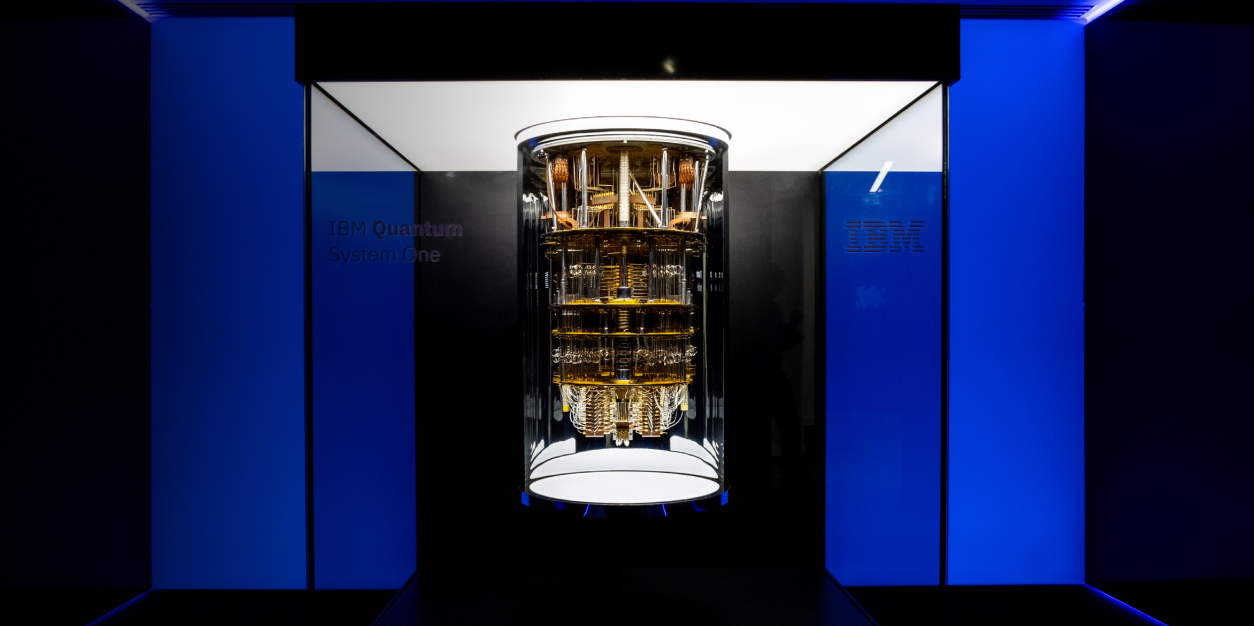
\includegraphics[width=0.7\linewidth]{SystemOne}
	\caption{IBM Q System One}
	\label{fig:systemone}
\end{figure}


\section{Nehézségek}
Mint láttuk, a kvantumszámítógépek jelenleg is kísérletezés alatt állnak, valamint számos kihívások továbbra is feltáratlanok maradtak. Egy kvantumszámítógép építése és karbantartása, azok speciális igényük és építőelemeik miatt mai napig nagy költségeket ölelnek fel.

A kvantumbitek minősége és stabilitása szintén egy jelentős probléma. A jelenlegi kvantumszámítógépek kevés qubittel rendelkeznek, skálázhatóságuk limitált, emiatt szűk körben használhatóak, számos komplex feladat megoldására továbbra is képtelenek.

Környezetre való érzékenysége miatt, extrém környezetekben tárolják őket. Az olyan tényezők, mint például a zaj, számítási problémákat okozhat, amik kijavítása rendkívül időigényes.

\section{Előnyök és veszélyek}
Nehézségei ellenére a kvantumszámítógépek számos lehetőséget is hordoznak magukban. Sokszor viszont ezek az előnyök rossz kezekben képesek veszélyeket is okozni.

Legfontosabb potenciáljuk a gyorsaságuk. Egy kvantumszámítógép sokkal gyorsabban képes elvégezni számításokat, mint a klasszikus számítógépek. Ez annak köszönhető, hogy egy klasszikus számítógép szekvenciálisan végzi feladatait, ezzel szemben a kvantumszámítógépek párhuzamosságra képesek.

Bár számos komplex feladat megoldására jelenleg is képtelenek, léteznek olyan összetettebb problémák, amiben a kvantumszámítógépek megfelelőnek bizonyultak, míg a klasszikus számítógépek számára megoldhatatlanok voltak. Ilyenek például különböző optimalizálási problémák, illetve faktoriális számítás. Ezek mögött számos kvantumalgoritmus jelenik meg, amely hasonlóan egy új ága a kvantuminformatikának.

A gyorsasági és számítási előnyei miatt több más iparág segítésére is szolgálhatnak a kvantumszámítógépek, többek között az anyag- és a gyógyszerkutatás is ide tartozik.

Viszont ezek az előnyök veszélyeket is hordozhatnak magukban. A már említett Shor algoritmus egy szám prímtényezős felbontását végzi el hatékonyan. A problémát az okozza, hogy a jelenlegi titkosítási algoritmusok (például az RSA) nagy része emiatt védtelen lesz, mivel ezek prímszámokat használnak titkosításra. Természetesen ezekre a problémákra is léteznek kutatások, így született a kvantumkriptográfia területe, ami fejlettebb biztonságot ígér.

A sok új lehetőség és a felsorolt előnyök nem léteznének a kvantum logikai kapuk nélkül, amik az alapkövei a kvantumszámítógépeknek.

\chapter{Klasszikus- és kvantum logikai kapuk}
\section{Klasszikus logikai kapuk és áramkörök}
Elektromos impulzusokhoz értékeket társítunk, az alapján hogy küldtünk-e vagy sem. Ha érzékelünk, akkor ezt I logikai értéknek vagy 1 bitnek tekintjük. Ellenkező esetben H logikai értéknek, vagy 0 bitnek feleltetjük meg.

Ezekhez az impulzusokhoz többnyire logikai kapukat társítunk, melyek bináris operátorokat foglalnak magukban. A logikai kapuk alapvető építőkövei az elektronikának és számos célra használják őket. Összekapcsolásukkal áramköröket alakíthatunk ki, amik lineárisak és balról jobbra értelmezzük őket. A bal oldali vezetékek jelentik a bemenetet, míg a jobb oldaliak a kimenetet. Az ismertebb kapukhoz speciális ábrák és igazságtáblák tartoznak.

Az igazságtáblák a klasszikus logika alapvető eszközei, amelyek segítségével értelmezhetjük az adott műveleteket, valamint ellenőrizhetjük áramköreinket. Megmutatják az összes lehetséges bemeneti kombinációt, illetve a műveletek alkalmazása után a várható kimenetet is. Ezek a logikai műveleteket, kifejezéseket Boole-algebrának nevezzük, amely egy 19. századi matematikus, George Boole nevét viseli
\subsection{Logikai kapuk}
\subsubsection{Buffer}
A buffer kapuk kimenete megegyezik a kimenetükkel, egy biten értelmezzük. Jele: $A$

\begin{figure}[H]
	\centering
	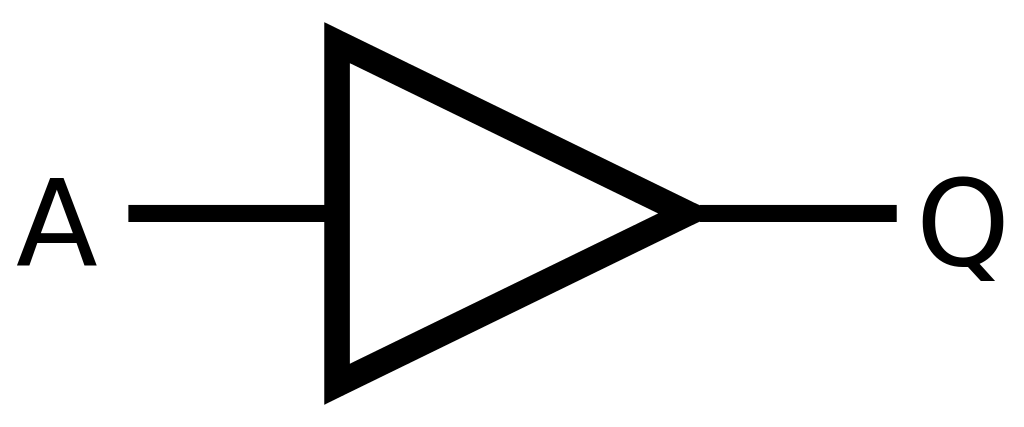
\includegraphics[width=0.3\linewidth]{buffer}
	\caption{Buffer kapu rajza}
	\label{fig:buffer}
\end{figure}


\begin{table}[H]
	\centering
	\begin{tabular}{c|c}
		$A$ & $A$\\
		\hline
		0 & 0\\
		1 & 1
	\end{tabular}
	\caption{Buffer kapu igazságtáblája}
\end{table}

\subsubsection{NOT, vagy Negáció}
A negáció kapu (vagy NOT) hasonlóan egy bites, a bemeneti jel logikai értékét megfordítja a kimeneten. Jele:$\neg A$

\begin{figure}[H]
	\centering
	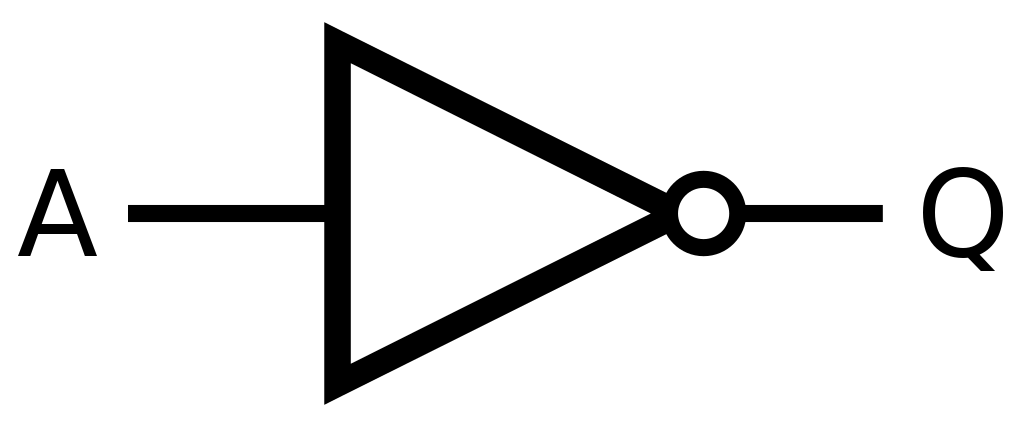
\includegraphics[width=0.3\linewidth]{not}
	\caption{NOT kapu rajza}
	\label{fig:not}
\end{figure}


\begin{table}[H]
	\centering
	\begin{tabular}{c|c}
		$A$ & $\neg A$\\
		\hline
		0 & 1\\
		1 & 0 
	\end{tabular}
	\caption{Negáció kapu igazságtáblája}
\end{table}

\subsubsection{AND, vagy Konjukció}
Más néven logikai és. Kétbites művelet, kimenete akkor igaz, ha mind a két operandusa igaz. Jele: $A \land B$

\begin{figure}[H]
	\centering
	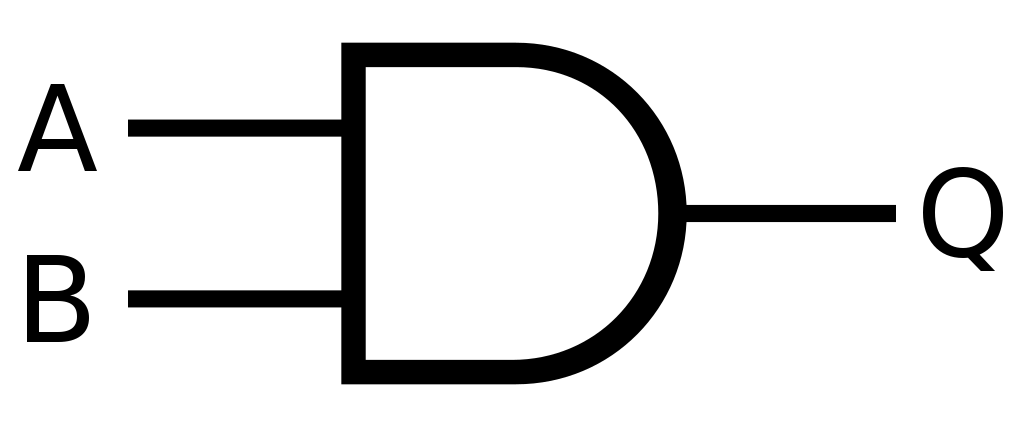
\includegraphics[width=0.3\linewidth]{and}
	\caption{AND kapu rajza}
	\label{fig:and}
\end{figure}


\begin{table}[H]
	\centering
	\begin{tabular}{c|c|c}
		$A$ & $B$ & $A \land B$\\               
		\hline
		0 & 0 & 0\\
		0 & 1 & 0\\
		1 & 0 & 0\\
		1 & 1 & 1
	\end{tabular}
	\caption{A konjukció igazságtáblája}
\end{table}

\subsubsection{OR, vagy Diszjunkció}
Más néven logikai vagy. Szintén kétbites művelet, értéke csak akkor hamis, ha mind a két operandusa hamis. Jele: $A \lor B$

\begin{figure}[H]
	\centering
	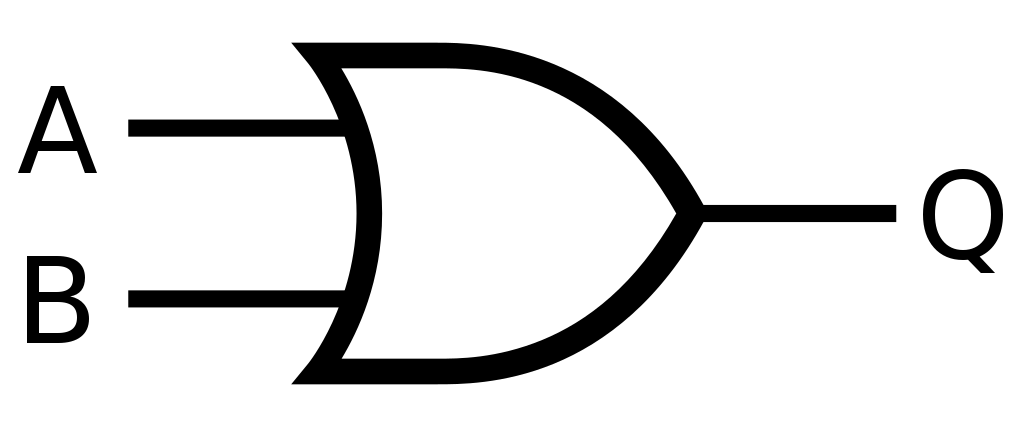
\includegraphics[width=0.3\linewidth]{or}
	\caption{OR kapu rajza}
	\label{fig:or}
\end{figure}


\begin{table}[H]
	\centering
	\begin{tabular}{c|c|c}
		$A$ & $B$ & $A \lor B$\\               
		\hline
		0 & 0 & 0\\
		0 & 1 & 1\\
		1 & 0 & 1\\
		1 & 1 & 1
	\end{tabular}
	\caption{A diszjunkció igazságtáblája}
\end{table}

\subsubsection{NAND, vagy Negált konjukció}
A konjukció negált változata, értéke akkor hamis, ha mindkét operandusa igaz. Jele: $\neg(A \land B)$

\begin{figure}[H]
	\centering
	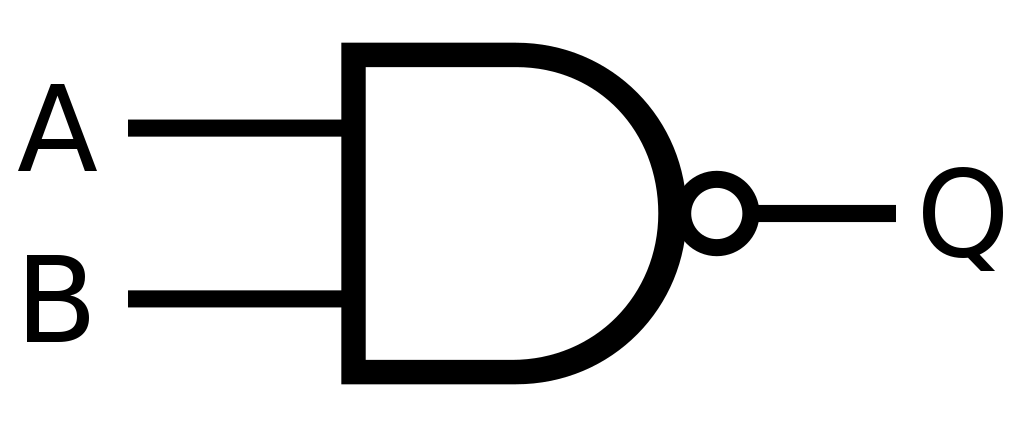
\includegraphics[width=0.3\linewidth]{nand}
	\caption{NAND kapu rajza}
	\label{fig:nand}
\end{figure}


\begin{table}[H]
	\centering
	\begin{tabular}{c|c|c}
		$A$ & $B$ & $\neg(A \land B)$\\               
		\hline
		0 & 0 & 1\\
		0 & 1 & 1\\
		1 & 0 & 1\\
		1 & 1 & 0
	\end{tabular}
	\caption{A negált konjukció igazságtáblája}
\end{table}

\subsubsection{NOR, vagy Negált diszjunkció}
A diszjunkció negált változata, értéke akkor igaz, ha mindkét operandusa hamis. Jele: $\neg(A \lor B)$

\begin{figure}[H]
	\centering
	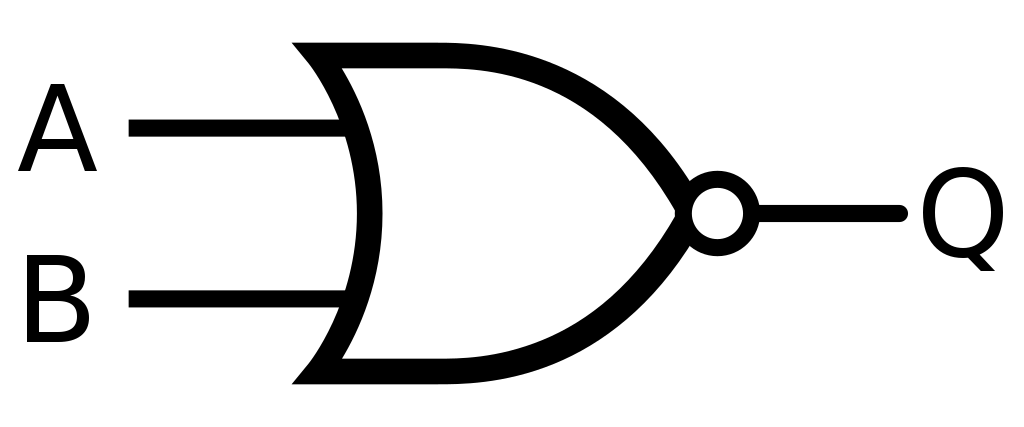
\includegraphics[width=0.3\linewidth]{nor}
	\caption{NOR kapu rajza}
	\label{fig:nor}
\end{figure}


\begin{table}[H]
	\centering
	\begin{tabular}{c|c|c}
		$A$ & $B$ & $\neg(A \lor B)$\\               
		\hline
		0 & 0 & 1\\
		0 & 1 & 0\\
		1 & 0 & 0\\
		1 & 1 & 0
	\end{tabular}
	\caption{A negált diszjunkció igazságtáblája}
\end{table}


\subsubsection{XOR, vagy Exclusive OR}
Más néven kizáró vagy. Értéke akkor hamis, ha a bemenetek megegyeznek. Jele: $A \oplus B$

\begin{figure}[H]
	\centering
	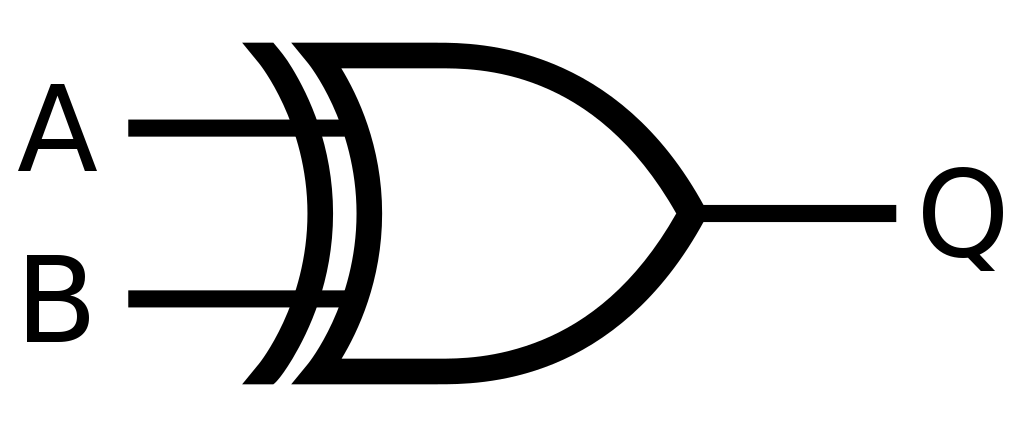
\includegraphics[width=0.3\linewidth]{xor}
	\caption{XOR kapu rajza}
	\label{fig:xor}
\end{figure}


\begin{table}[H]
	\centering
	\begin{tabular}{c|c|c}
		$A$ & $B$ & $A \oplus B$\\               
		\hline
		0 & 0 & 0\\
		0 & 1 & 1\\
		1 & 0 & 1\\
		1 & 1 & 0
	\end{tabular}
	\caption{A negált konjukció igazságtáblája}
\end{table}


\subsubsection{XNOR, vagy Exclusive NOR}
A kizáró vagy negáltja, értéke akkor hamis, ha a bemenetek különböznek Jele: $\neg (A \oplus B)$

\begin{figure}[H]
	\centering
	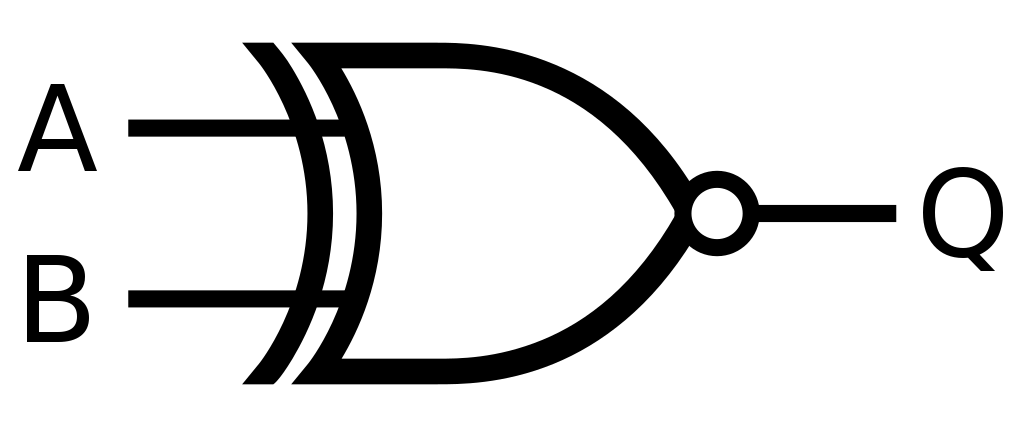
\includegraphics[width=0.3\linewidth]{xnor}
	\caption{XNOR kapu rajza}
	\label{fig:xnor}
\end{figure}


\begin{table}[H]
	\centering
	\begin{tabular}{c|c|c}
		$A$ & $B$ & $\neg (A \oplus B)$\\               
		\hline
		0 & 0 & 1\\
		0 & 1 & 0\\
		1 & 0 & 0\\
		1 & 1 & 1
	\end{tabular}
	\caption{A negált konjukció igazságtáblája}
\end{table}

\subsection{Univerzális kapuk}
Léteznek olyan logikai kapuk, amelyek képesek reprodukálni bármely másik működését. Ezek az univerzális kapuk lehetővé teszik akármelyik logikai függvény leképezését, ami azt jelenti, hogy akár tetszőleges áramkör is megvalósítható velük.

Bizonyítható, hogy bármilyen logikai függvény összeállítható csak NOT és AND, vagy NOT és OR függvények kombinációival. Mint láttuk, ezek a kapuk ötvözhetőek, erre szolgálnak a NAND és NOR kapuk.

Ebből következtethető, hogy bármilyen Boole-függvény megvalósítható olyan áramkörrel, amely csak NAND vagy NOR kapukat alkalmaz. Gyakran emiatt előnyt élveznek, mivel más kapuknak nincs ilyen tulajdonsága.

\section{Kvantum logikai kapuk és áramkörök}
A kvantumkapuk jelentőségét a kvantummechanika alapelveire támaszkodva értelmezhetjük, amelyek olyan jelenségeket és viselkedéseket írnak le, melyek a klasszikus fizika keretein belül nem megfigyelhetők vagy magyarázhatók. A kvantummechanika alapján működő kapuk és áramkörök lehetővé teszik olyan számítások végrehajtását, amelyek rendkívül nagy számítási kapacitással és párhuzamosítással rendelkeznek, ami jelentős előnyöket kínál a hagyományos, klasszikus számítógépekkel szemben.

Bár vannak hasonlóságok a klasszikus változatokhoz képest, a kvantum logikai kapuk egy sokkal komplexebb matematikai hátteret és fizikai jelenségeket hordoznak magukban.

Jelen alfejezet csak pár, ismertebb logikai kaput tartalmaz, de fontos megemlíteni, hogy a kvantumkapuk száma végtelen. Mivel szakdolgozatom az egyqubites kapukra irányul, ezért a több kvantumbites változatok csak megemlítő jelleggel szerepelnek.

\subsection{Qubit}
A kvantumbit, röviden qubit, a kvantuminformatika alapvető építőeleme, és a klasszikus számítógépek működésétől eltérő, kvantummechanikai alapokon nyugvó adatábrázolási egység. Míg a hagyományos bit csak két állapotban (0 vagy 1) lehet jelen, a qubit képes egyszerre számos állapotban lenni, ami egyike annak a tulajdonságának, amely a kvantuminformatikát annyira különlegessé teszi.

\begin{figure}[H]
	\centering
	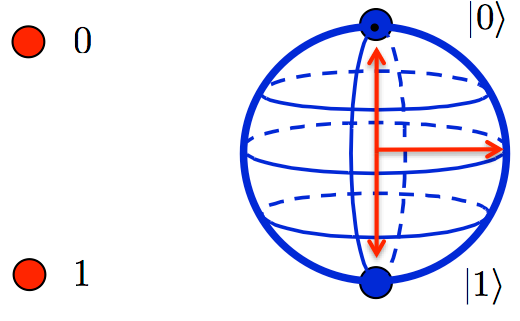
\includegraphics[width=0.3\linewidth]{bitQubit}
	\caption{A bit és qubit reprezentációja}
	\label{fig:bitqubit}
\end{figure}

Ahogy az \az{\ref{fig:bitqubit}}.~ábrán látható, a qubit számos állapotát egy úgynevezett Bloch gömbön ábrázoljuk, északi pólusán $\ket{0}$, déli pólusán pedig $\ket{1}$ helyezkedik el. A $\ket{}$ és $\bra{}$ jelöléseket braket-nek nevezzük, de Dirac jelölésként is ismert, és a kvantumállapotok jelölésében segít. A ket ($\ket{\Psi}$) egy oszlopvektort, a bra ($\bra{\Psi}$) pedig egy sorvektort jelöl.

A kvantummechanika alapelvei és a qubitok sajátos tulajdonságai lehetővé teszik
olyan számítási feladatok elvégzését, amelyek a hagyományos számítógépek számára gyakorlatilag lehetetlenek lennének.

\subsection{Szuperpozíció és összefonódás}

Egy qubit állapotát a következőképpen adhatjuk meg:
\begin{equation}\label{qubitallapot}
	\ket{\Psi}=\alpha\ket{0}+\beta\ket{1},
\end{equation}
ahol $\alpha$ és $\beta$ komplex számok, valamint teljesül, hogy $|\alpha|^2+|\beta|^2=1$. Ez azt jelenti, hogy a $\ket{\Psi}$ kvantumbit $|\alpha|^2$ eséllyel 0, $|\beta|^2$-el pedig 1 lesz. Ezt szuperpozíciónak nevezzük. A két szélső érték, azaz $\ket{0}$ vagy $\ket{1}$ akkor áll elő, ha $\alpha$ 0 vagy 1, $\beta$ pedig ennek ellentettje. A szuperpozíció legjobban a Schrödinger macskája gondolatkísérlettel prezentálható, melyet Erwin Schrödinger fogalmazott meg 1935-ben.

A qubit másik fontos jelensége a kvantum-összefonódás. Ez egy olyan jelenség a kvantummechanikában, amelyben két vagy több részecske állapota olyan összekapcsolt módon van, hogy az egyiken végzett mérések azonnal hatnak a másikra, függetlenül attól, hogy a részecskék milyen fizikai távolságra vannak egymástól.

\subsection{Qubit mérése}
Méréskor eredményként egyetlen klasszikus bitet kapunk. A qubit mérése során az eredmény kvantumállapota "összeomlik" az adott értékre, amelyet a mérés során megfigyeltünk. Azaz elveszti a szuperpozícióját és az összefonódottságát, ami azt jelenti, hogy a mérés után a rendszer elveszíti a kvantumos jellegét, és klasszikus állapotba kerül. Ez az összeomlás a kvantummechanika alapvető jelensége, amely lehetővé teszi a kvantumrendszer állapotának rögzítését a mérés pillanatában. Emiatt a mérések kritikus szerepet játszanak.

\begin{figure}[H]
	\centering
	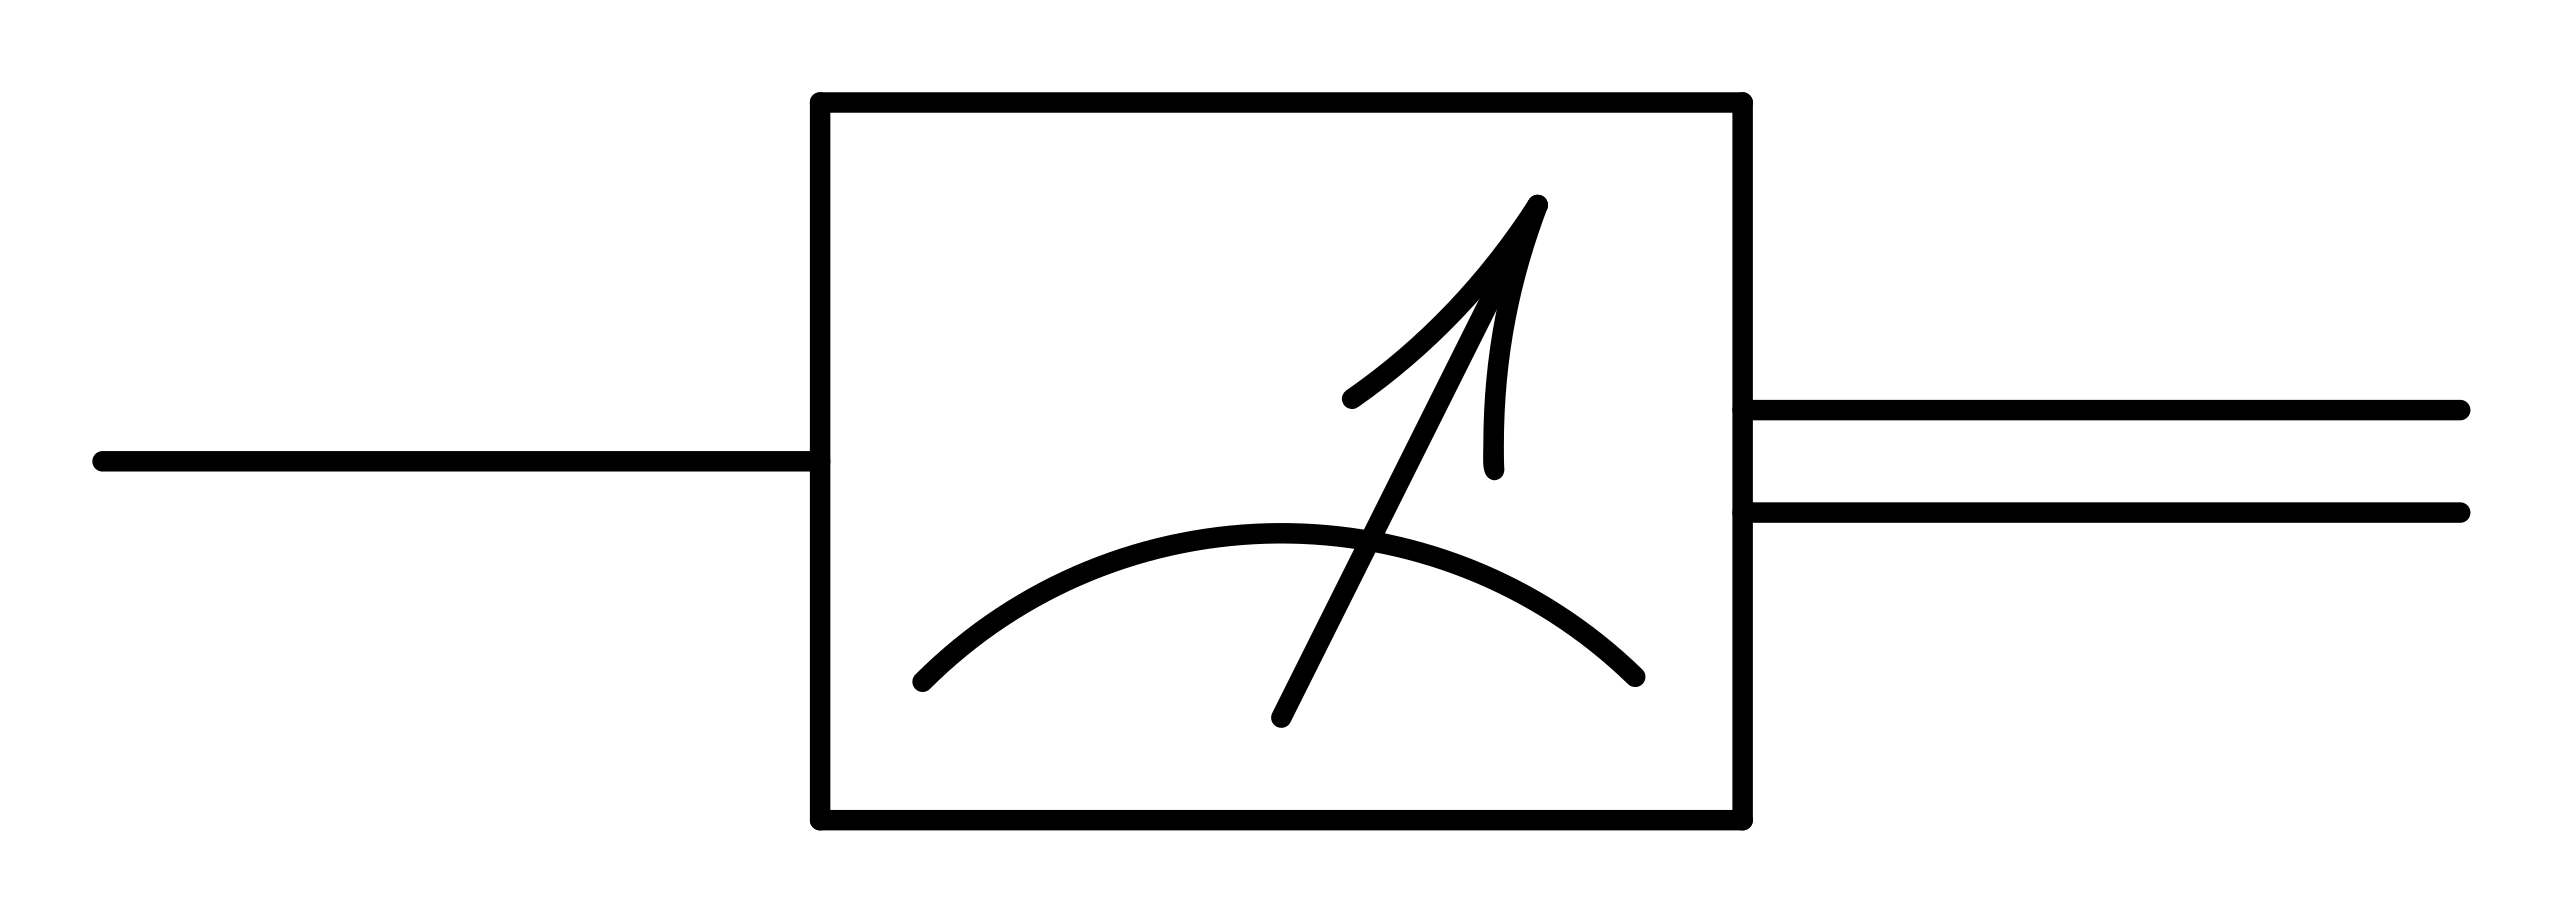
\includegraphics[width=0.3\linewidth]{measure}
	\caption{Mérés rajza}
	\label{fig:measure}
\end{figure}

\subsection{Kvantum logikai kapuk}\label{kvantumkapuk}

\subsubsection{I, vagy Identity}
A buffer kapuhoz hasonlóan nem végez műveletet, helyben hagyja a kvantumbiteket. Egy qubiten használjuk. Azonosság transzformációként működik, alakja:

\begin{equation}
	I= 
	\begin{bmatrix}
		1 & 0\\
		0 & 1
	\end{bmatrix}
\end{equation}

Ez egy tetszőleges kvantumbiten:

\begin{equation}
	\ket{\Psi}=I\ket{\varphi}
		\begin{bmatrix}
			1 & 0\\
			0 & 1
		\end{bmatrix}
		\begin{bmatrix}
			a\\
			b
		\end{bmatrix}=a\ket{0}+b\ket{1}
\end{equation}


\begin{figure}[H]
	\centering
	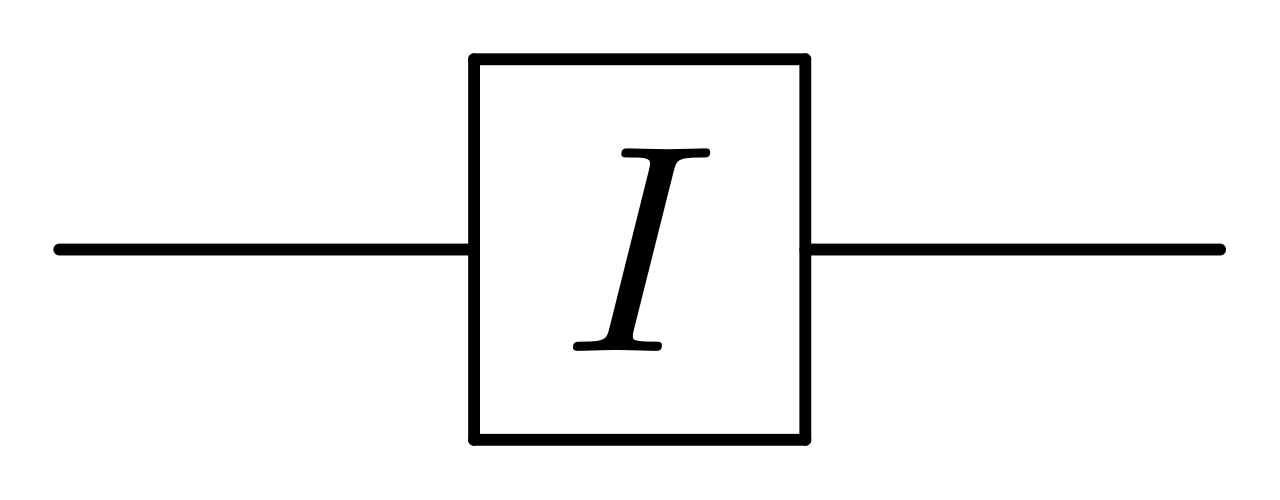
\includegraphics[width=0.3\linewidth]{Identity}
	\caption{I kapu rajza}
	\label{fig:identity}
\end{figure}


\subsubsection{X, vagy Pauli-X}
A klasszikus NOT kapunak felel meg, bit-flipnek is hívják. A Bloch gömb $X$ tengelyére tükröz. Egy qubiten működik. Alakja:

\begin{equation}
	X= 
	\begin{bmatrix}
		0 & 1\\
		1 & 0
	\end{bmatrix}
\end{equation}

Ez egy tetszőleges kvantumbiten:

\begin{equation}
	\ket{\Psi}=X\ket{\varphi}
		\begin{bmatrix}
			0 & 1\\
			1 & 0
		\end{bmatrix}
		\begin{bmatrix}
			a\\
			b
		\end{bmatrix}=b\ket{0}+a\ket{1}
\end{equation}


Az X kapu hatására a valószínűségi amplitúdók cserélődnek. Inverze saját maga, tehát például:

\begin{equation}
	\ket{\Psi}=XX\ket{0}=\ket{0}
\end{equation}

\begin{figure}[H]
	\centering
	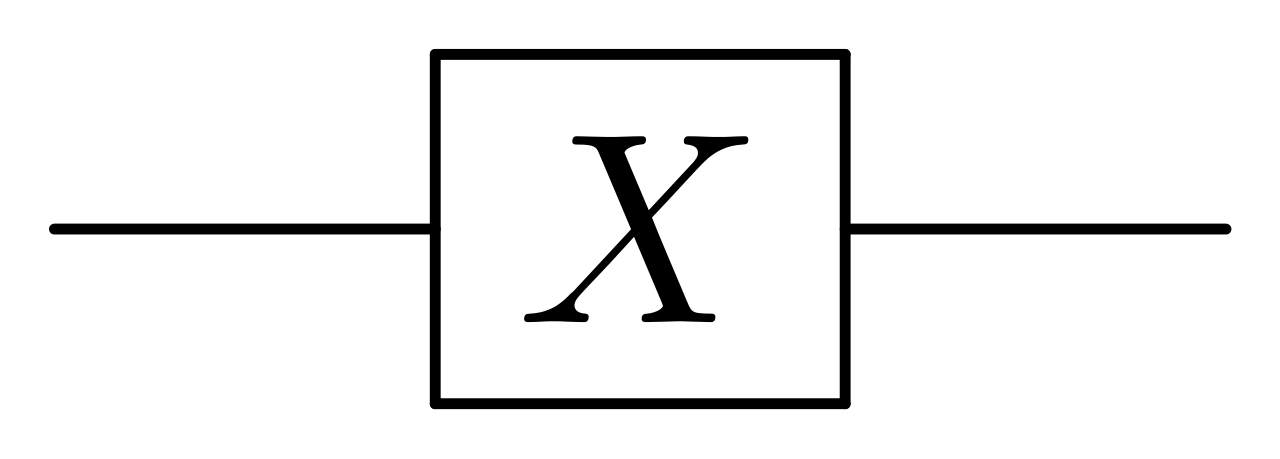
\includegraphics[width=0.3\linewidth]{Pauli_X}
	\caption{X kapu rajza}
	\label{fig:paulix}
\end{figure}


\subsubsection{Y, vagy Pauli-Y}
Az X kapuhoz hasonlóan felcseréli a $\ket{0}$-t és az $\ket{1}$-t, viszont az Y kapu a relatív fázist is megváltoztatja. A Bloch gömb $Y$ tengelyére tükröz. Egy qubiten működik. Alakja:

\begin{equation}
	Y= 
	\begin{bmatrix}
		0 & -i\\
		i & 0
	\end{bmatrix}
\end{equation}

Ez egy tetszőleges kvantumbiten:

\begin{equation}
	\ket{\Psi}=Y\ket{\varphi}
		\begin{bmatrix}
			0 & -i\\
			i & 0
		\end{bmatrix}
		\begin{bmatrix}
			a\\
			b
		\end{bmatrix}=-ib\ket{0}+ia\ket{1},
\end{equation}

ahol $i$ komplex szám. Inverze saját maga, tehát például:

\begin{equation}
	\ket{\Psi}=YY\ket{0}=\ket{0}
\end{equation}

\begin{figure}[H]
	\centering
	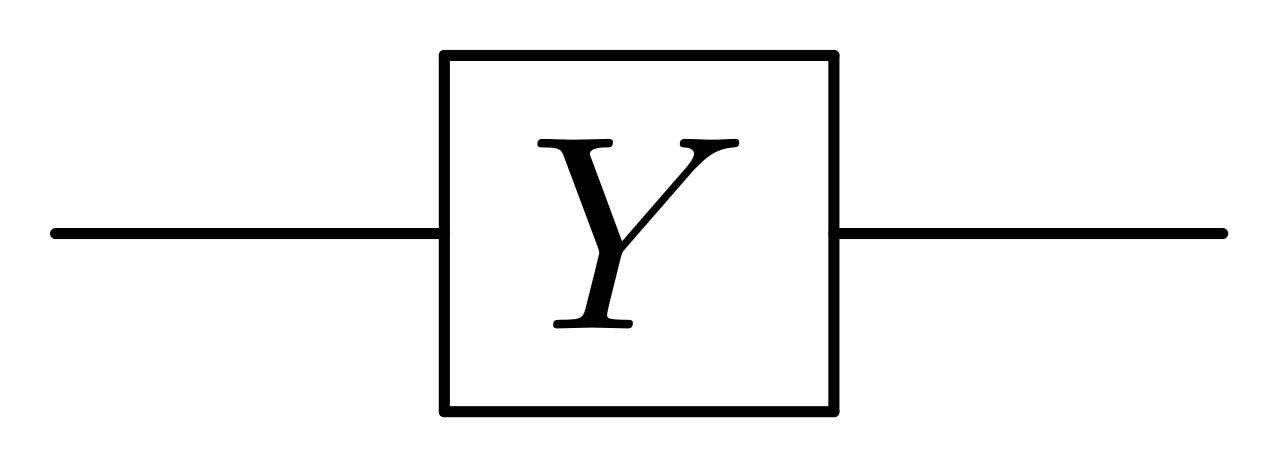
\includegraphics[width=0.3\linewidth]{Pauli_Y}
	\caption{Y kapu rajza}
	\label{fig:pauliy}
\end{figure}


\subsubsection{Z, vagy Pauli-Z}
Phase-flip kapunak is hívják, ebből adódóan a fázist cseréli meg. A Bloch gömb $Z$ tengelyére tükröz. Egy qubiten működik. Alakja:

\begin{equation}
	Z= 
	\begin{bmatrix}
		1 & 0\\
		0 & -1
	\end{bmatrix}
\end{equation}

Ez egy tetszőleges kvantumbiten:

\begin{equation}
	\ket{\Psi}=Z\ket{\varphi}
		\begin{bmatrix}
			1 & 0\\
			0 & -1
		\end{bmatrix}
		\begin{bmatrix}
			a\\
			b
		\end{bmatrix}=a\ket{0}-b\ket{1}
\end{equation}

Látható, hogy a Z kapu csak az $\ket{1}$ valószínűségi amplitúdót változtatja. Inverze saját maga, tehát például:

\begin{equation}
	\ket{\Psi}=ZZ\ket{0}=\ket{0}
\end{equation}

\begin{figure}[H]
	\centering
	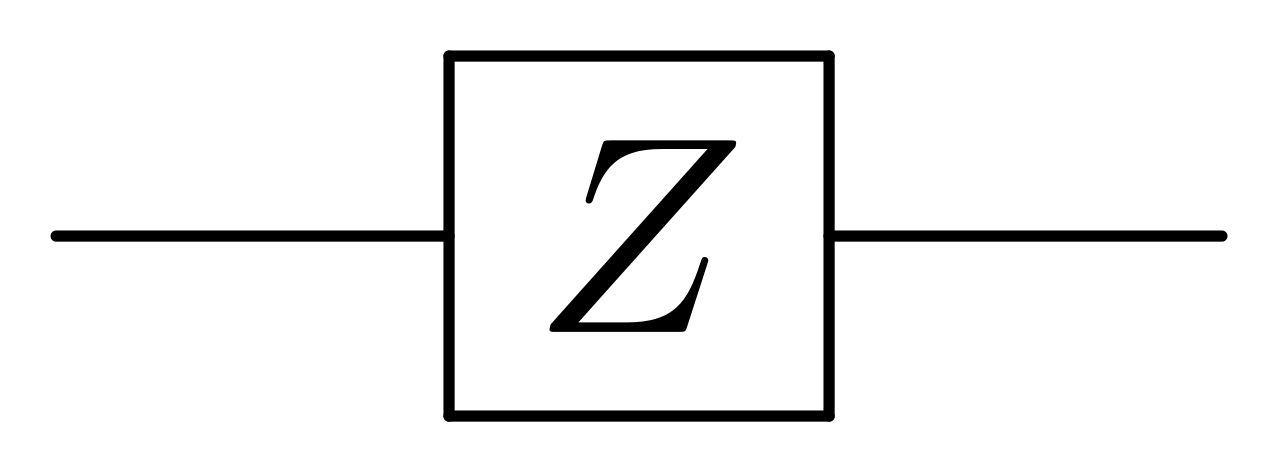
\includegraphics[width=0.3\linewidth]{Pauli_Z}
	\caption{Z kapu rajza}
	\label{fig:pauliz}
\end{figure}

\subsubsection{H, vagy Hadamard}
A Hadamard kapu segítségével a már említett szuperpozíciós állapotokat lehet előállítani. Egy qubiten működik. Alakja:

\begin{equation}
	H= \frac{1}{\sqrt{2}}
	\begin{bmatrix}
		1 & 1\\
		1 & -1
	\end{bmatrix}
\end{equation}

Ez egy tetszőleges kvantumbiten:

\begin{equation}
	\ket{\Psi}=H\ket{\varphi}=\frac{1}{\sqrt{2}}
	\begin{bmatrix}
		1 & 1\\
		1 & -1
	\end{bmatrix}
	\begin{bmatrix}
		a\\
		b
	\end{bmatrix}=\frac{a+b}{\sqrt{2}}\ket{0}+\frac{a-b}{\sqrt{2}}\ket{1}
\end{equation}

Mivel a kaput gyakran használják a standard bázisvektorokon, emiatt külön számon tartják őket:

\begin{equation}
	\ket{\Psi}=H\ket{0}=\frac{1}{\sqrt{2}}
	\begin{bmatrix}
		1 & 1\\
		1 & -1
	\end{bmatrix}
	\begin{bmatrix}
		1\\
		0
	\end{bmatrix}=\frac{\ket{0}+\ket{1}}{\sqrt{2}}
\end{equation}

\begin{equation}
	\ket{\Psi}=H\ket{1}=\frac{1}{\sqrt{2}}
	\begin{bmatrix}
		1 & 1\\
		1 & -1
	\end{bmatrix}
	\begin{bmatrix}
		0\\
		1
	\end{bmatrix}=\frac{\ket{0}-\ket{1}}{\sqrt{2}}
\end{equation}

A Hadamard kapu inverze saját maga, tehát például:

\begin{equation}
	\ket{\Psi}=HH\ket{0}=\ket{0}
\end{equation}

\begin{figure}[H]
	\centering
	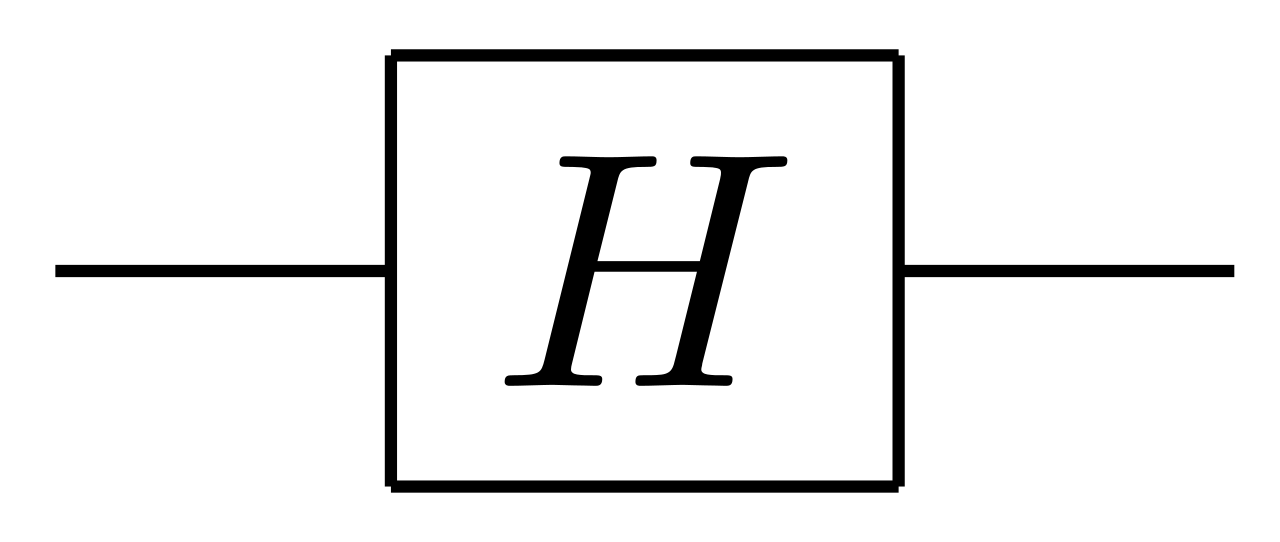
\includegraphics[width=0.3\linewidth]{Hadamard}
	\caption{H kapu rajza}
	\label{fig:hadamard}
\end{figure}


\subsubsection{S, vagy Phase}
Más néven fáziseltolási kapu. $\pi/2$ fáziseltolást alkalmaz a qubit állapotára. A Bloch gömb körül az óramutató járásával megegyező irányban forgat $\pi/2$ radiánnal. Egy qubiten működik. Alakja:

\begin{equation}
	S= 
	\begin{bmatrix}
		1 & 0\\
		0 & -i
	\end{bmatrix}
\end{equation}

Ez egy tetszőleges kvantumbiten:

\begin{equation}
	\ket{\Psi}=S\ket{\varphi}=
	\begin{bmatrix}
		1 & 0\\
		0 & -i
	\end{bmatrix}
	\begin{bmatrix}
		a\\
		b
	\end{bmatrix}=a\ket{0}-ib\ket{1}
\end{equation}

\begin{figure}[H]
	\centering
	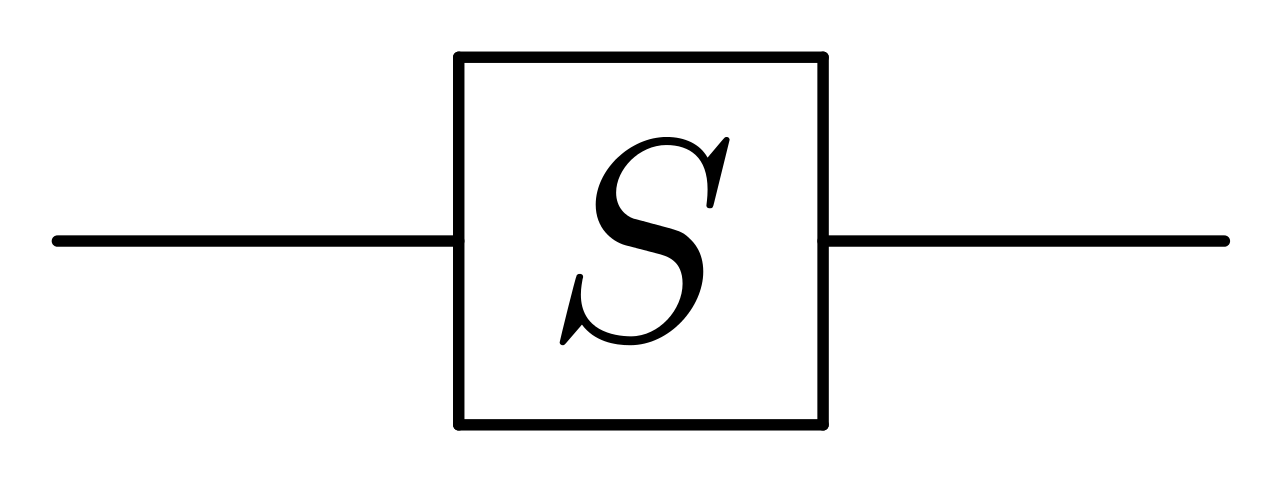
\includegraphics[width=0.3\linewidth]{Qcircuit_S.svg}
	\caption{S kapu rajza}
	\label{fig:qcircuits}
\end{figure}


\subsubsection{T, vagy $\pi/8$}
A T kapu, hasonlóan az S kapuhoz, fáziseltolást alkalmaz egy qubit állapotára. Az állapotvektort $\pi/4$ radiánnal forgat a Bloch gömb körül, óramutató járással megegyező irányban. Alakja:

\begin{equation}
	T= 
	\begin{bmatrix}
		1 & 0\\
		0 & e^{i\pi/4}
	\end{bmatrix}
\end{equation}

Ez egy tetszőleges kvantumbiten:

\begin{equation}
	\ket{\Psi}=T\ket{\varphi}=
	\begin{bmatrix}
		1 & 0\\
		0 & e^{i\pi/4}
	\end{bmatrix}
	\begin{bmatrix}
		a\\
		b
	\end{bmatrix}=a\ket{0}+e^{i\pi/4}b\ket{1}
\end{equation}

Az S kapuval való azonosságok miatt elmondható, hogy $S=T^{2}$

\begin{figure}[H]
	\centering
	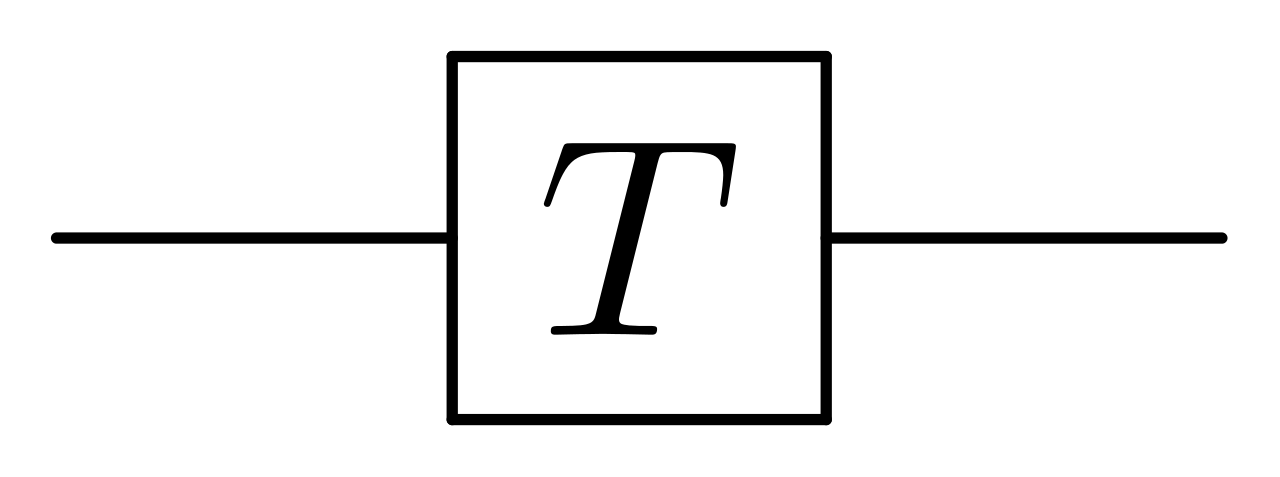
\includegraphics[width=0.3\linewidth]{Qcircuit_T.svg}
	\caption{T kapu rajza}
	\label{fig:qcircuitt}
\end{figure}


\subsubsection{CNOT, vagy Controlled Not}
A CNOT kapu két qubites művelet, ahol az első qubit vezérlő-, a második pedig cél kvantumbit néven ismert. Ha a vezérlő $\ket{1}$, akkor a cél qubiten X kaput használ, a többi változatlan. Amennyiben a vezérlő qubit $\ket{0}$, a cél változatlan marad. Klasszikus logikai kapuként is alkalmazható. Inverze saját maga. Alakja:

\begin{equation}
	CNOT= 
	\begin{bmatrix}
		1 & 0 & 0 & 0\\
		0 & 1 & 0 & 0\\
		0 & 0 & 0 & 1\\
		0 & 0 & 1 & 0
	\end{bmatrix}
\end{equation}

\begin{figure}[H]
	\centering
	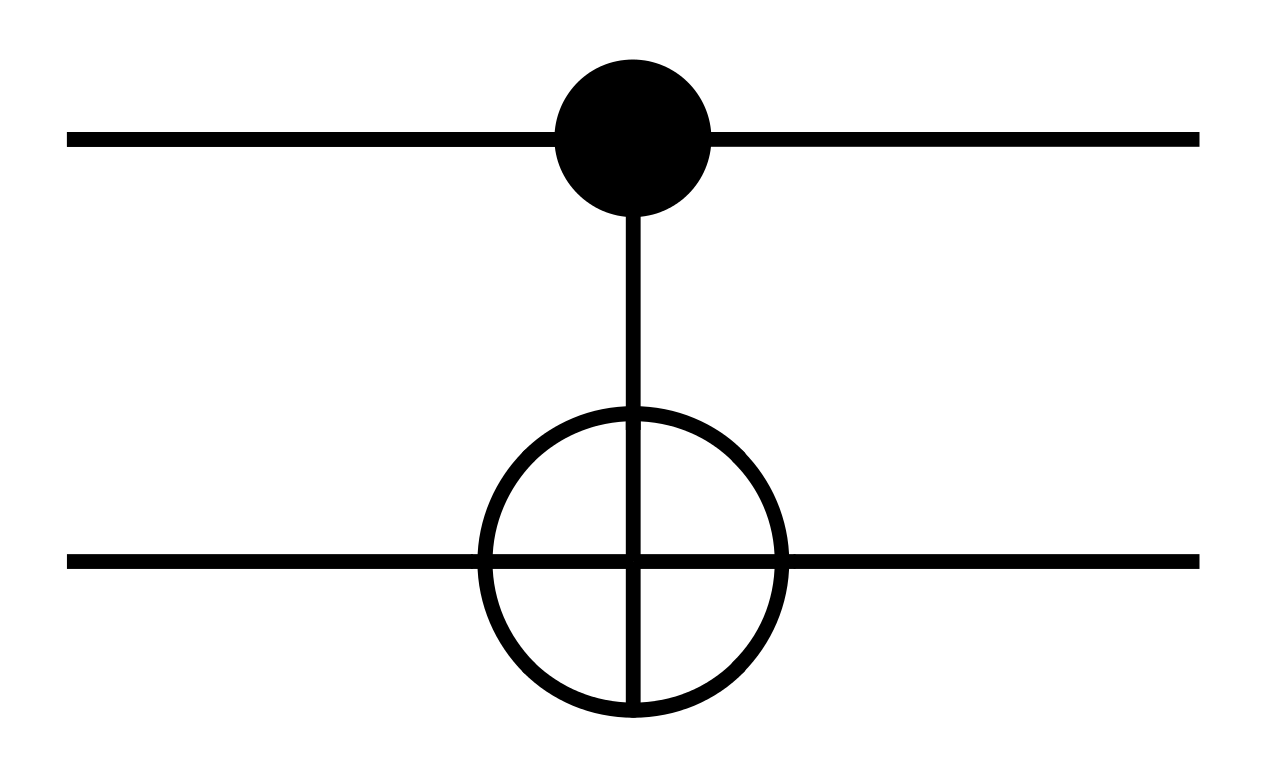
\includegraphics[width=0.25\linewidth]{CNOT}
	\caption{CNOT kapu rajza}
	\label{fig:cnot}
\end{figure}


\subsubsection{SWAP}
Két qubites kvantumkapu, mely felcseréli a bemenetek állapotát. Mivel három CNOT kapuval valósítható meg, így más jelölést is alkalmaznak rá, az egyszerűbb változat \az{\ref{fig:swap}}.~ábrán látható. Inverze saját maga. Alakja:

\begin{equation}
	SWAP= 
	\begin{bmatrix}
		1 & 0 & 0 & 0\\
		0 & 0 & 1 & 0\\
		0 & 1 & 0 & 0\\
		0 & 0 & 0 & 1
	\end{bmatrix}
\end{equation}

\begin{figure}[H]
	\centering
	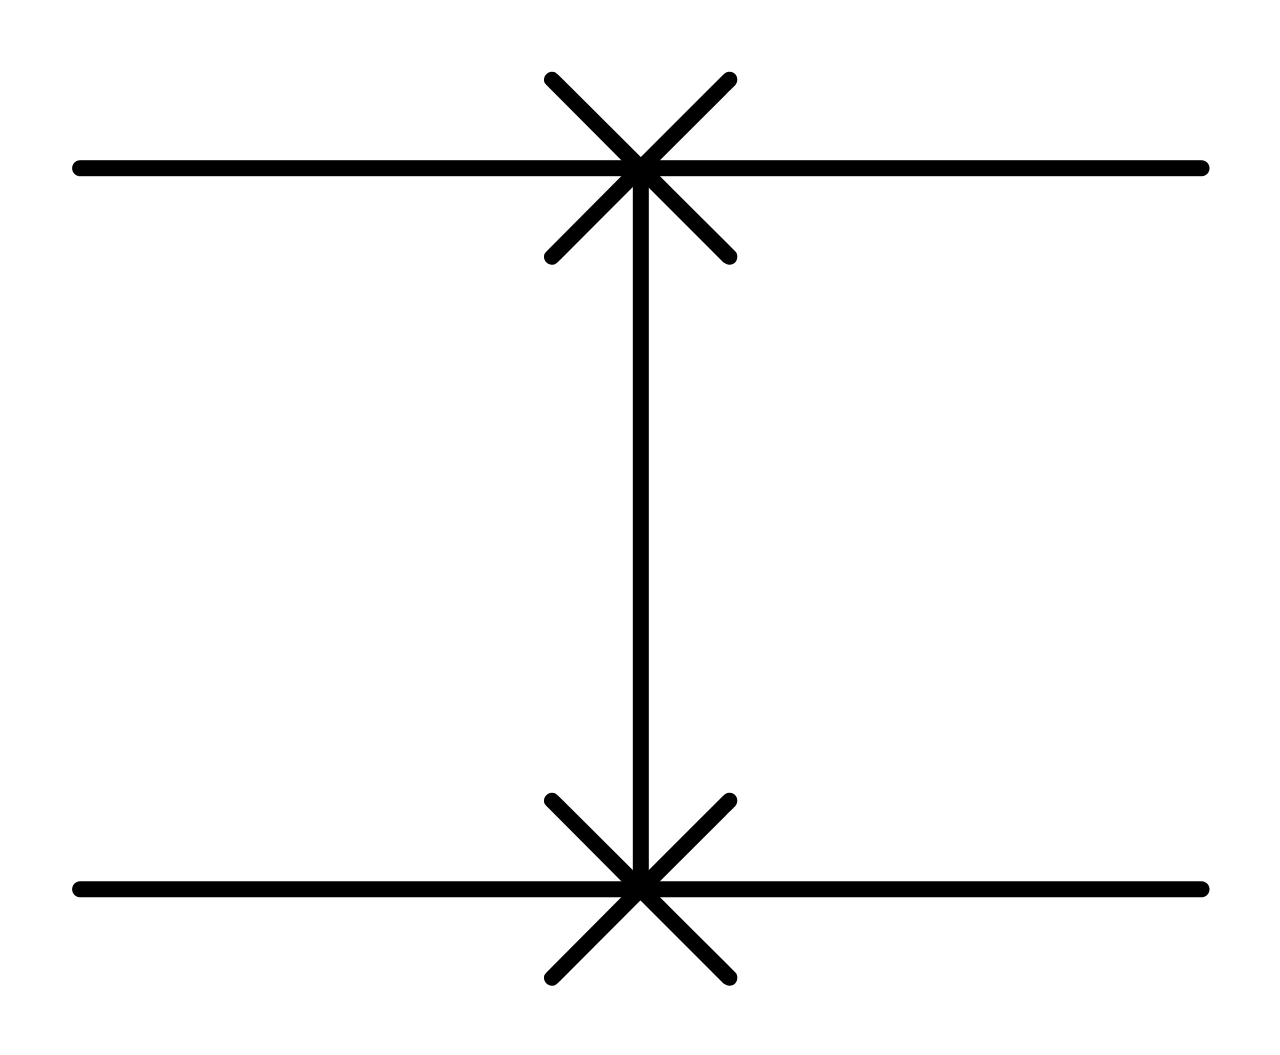
\includegraphics[width=0.25\linewidth]{SWAP}
	\caption{SWAP kapu rajza}
	\label{fig:swap}
\end{figure}


\subsubsection{Toffoli}
Ahogy az \az{\ref{fig:toffoligate}}.~ábrán látható, a Toffoli kapu CNOT műveletet használ, ezért szokás CCNOT kapunak is nevezni. Három qubiten működik, az első kettő vezérlő, az utolsó pedig a cél qubit. Klasszikus logikai kapuként is alkalmazható, ez esetben univerzális klasszikus kapunak tekintik. Inverze saját maga. Alakja:

\begin{equation}
	Toffoli= 
	\begin{bmatrix}
		1 & 0 & 0 & 0 & 0 & 0 & 0 & 0\\
		0 & 1 & 0 & 0 & 0 & 0 & 0 & 0\\
		0 & 0 & 1 & 0 & 0 & 0 & 0 & 0\\
		0 & 0 & 0 & 1 & 0 & 0 & 0 & 0\\
		0 & 0 & 0 & 0 & 1 & 0 & 0 & 0\\
		0 & 0 & 0 & 0 & 0 & 1 & 0 & 0\\
		0 & 0 & 0 & 0 & 0 & 0 & 0 & 1\\
		0 & 0 & 0 & 0 & 0 & 0 & 1 & 0\\
	\end{bmatrix}
\end{equation}

\begin{figure}[H]
	\centering
	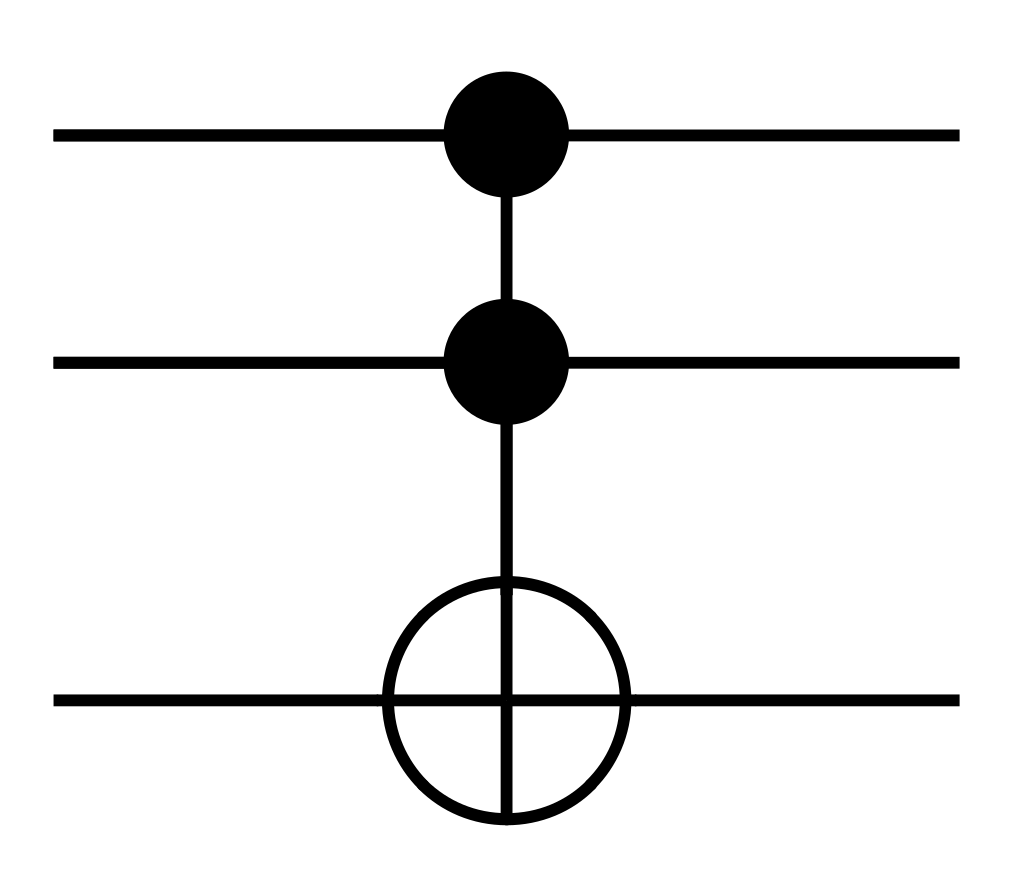
\includegraphics[width=0.25\linewidth]{Toffoli_gate.svg}
	\caption{Toffoli kapu rajza}
	\label{fig:toffoligate}
\end{figure}


\subsection{Univerzális kvantumkapuk}
Klasszikus esetben tapasztaltuk, hogy léteznek univerzális kapuk. Ez amiatt lehetséges, mivel csak végesen sok Boole-függvény van egy adott számú változó esetén. Kvantumkapuknál elmondható, hogy a lehetséges kapuk száma végtelen sok. Emiatt a fontos különbség miatt univerzális kvantumkapuk halmaza sem létezik. Ellenben, ha a kapuknak vesszük egy véges számú gyűjteményét, akkor beszélhetünk univerzális megoldásokról, viszont ezek sem használhatóak minden lehetséges kvantumáramkörre, csak hozzávetőlegesen.

\section{Reverzibilis kapuk}
Megfordítható kapuknak is nevezik őket. Két alapvető tulajdonsága van:
\begin{enumerate}
	\item Az eredményükből egyértelműen kikövetkeztethetőek a bemenetek, azaz egy bemeneti kombinációhoz pontosan egy kimeneti kombináció tartozik, és fordítva
	\item Lehetővé teszik a bemenetek helyreállítását a kimenetekből anélkül, hogy információt veszítenének.
\end{enumerate}

Vegyük például az OR kaput. Mint láttuk, értéke csak akkor hamis, ha bemenetei hamisak. Viszont minden más esetben nem tudjuk megállapítani, hogy melyik volt az aktuális bemenet a háromból, hacsak nincs további információnk. Tehát az OR kapuról elmondható, hogy irreverzibilis (nem reverzibilis) kapu. A legtöbb klasszikus logikai kapu szintén ebbe a csoportba tartozik, a már említett kapuk közül ez alól a CNOT és a Toffoli kivétel.

Lehetőség van klasszikus logikai művelet végrehajtására csak reverzibilis kapuk használatával, de ilyen esetekben gyakran szükségessé válik a segédbitek használata.

Alapvetően bármilyen reverzibilis klasszikus kapu megvalósítható kvantumszámítógépeken, így emiatt létezik a Toffoli és CNOT kapunak kvantum változata is.

A klasszikus logikai kapukkal ellentétben, a kvantum kapuk közül mindegyik reverzibilis.

\chapter{Tanulás segítő program és applikáció}
\section{Technológiai körültekintés}
A különböző technológiák és eszközök közötti választás nem mindig egyértelmű. Ezért szükséges részletesen mérlegelni és összehasonlítani az elérhető lehetőségeket. A nyelv, keretrendszer vagy platform kiválasztása előtt érdemes megfontolni a különböző szempontokat, mint például a teljesítmény, a fejlesztési idő és a támogatottság. Szakdolgozatom írásának kezdetekor, a nyelv és keretrendszer választásnál figyelembe vettem az alábbi elképzeléseket:
\begin{enumerate}
	\item Két részből álljon: egy telefonos applikációból és egy asztali alkalmazásból, mindkettő angol nyelven.
	\item Az egy kvantumbites kapuk egy csoportját mutassa be, ezeket interaktív, tanulást segítő formában.
	\item A telefonos applikáció képes legyen csatlakozni az asztali alkalmazásra, majd szenzor adatokat küldeni. Fontos volt továbbá, hogy rövid ismertetőket tudjon a felhasználó olvasni az adott kapukról.
	\item A program egy letisztult felületet nyújtson, ahol a felhasználó válogathat az adott egy kvantumbites kapuk közül. Ezekről kapja meg azt a leírást, ami a telefonon is elérhető, valamint animációkat is tudjon nézni róluk.
	\item A program középpontja egy Bloch gömb legyen, egy állapotvektorral. Ezt a felhasználó tudja állítani, valamint amennyiben csatlakoztatott telefont, ki is tudja próbálni az adott kapukat. A telefon forgatásával képes legyen a cél állapotba igazítani a vektort, ez egy minimális hibatűréssel történjen.
\end{enumerate}

A program lehetőségeit szűkítette a tény, hogy minél pontosabb ábrákat, reprezentációkat kellett keresnem. A gömb forgatását vettem a legmeghatározóbb tényezőnek választásnál. Egy egyszerű 3D-s objektumot több nyelv és keretrendszer is támogat. Kipróbáltam, hogy ez Java Fx-ben valamint  PythonQt-ban hogy jelenik meg. Viszont, mint ahogy azt \az{\ref{fig:bitqubit}}.~ábrán is látható, a Bloch gömb tartalmaz egy vektort, aminek pozíciója változhat, ami miatt a klasszikus megjelenítés nem elegendő, hiszen nem az objektumot forgatjuk. Emiatt fontos volt áttekintenem, hogy milyen kvantumáramkörökkel foglalkozó könyvtárakkal szolgálnak a keretrendszerek.

A telefonos applikáció kapcsán fontos volt, hogy a választott operációs rendszer minél több felhasználót lefedjen, valamint közel pontos szenzor adatot legyen képes küldeni.

\section{Választott technológiák}
\subsection{Asztali alkalmazás}
\subsubsection{Python}
A Python egy magas szintű, interpretált programozási nyelv, amely egyszerűségéről és könnyen olvashatóságáról ismert. Manapság a legnépszerűbb nyelv.

Szintaxisát úgy tervezték, hogy intuitív és olvasható legyen, így kezdők és tapasztalt programozók számára egyaránt nagyszerű választás. Hangsúlyozza a kód olvashatóságát, és lehetővé teszi a fejlesztők számára, hogy más nyelvekhez képest kevesebb kódsorban oldjanak meg problémákat.

A Python emellett egy interpreteres  nyelv, ami azt jelenti, hogy a Pythonban írt kód soronként hajtódik végre, nem pedig előzetesen gépi kódba fordítva. Ez megkönnyíti a fejlesztést és a hibakeresést, mivel a kód azonnal végrehajtható külön fordítási lépés nélkül.

Dinamikus típusrendszerének köszönhetően, változótípusokra a rendszer futás közben következtet. Ez nagyobb rugalmasságot és gyorsabb fejlesztést tesz lehetővé.

A Python támogatja az objektum-orientált programozás (OOP) elveit, lehetővé téve a fejlesztők számára, hogy osztályokat és objektumokat hozzanak létre az adatok és a viselkedések egységbe zárásához.

Egy átfogó könyvtárral is rendelkezik, amely modulokat és funkciókat biztosít különféle feladatok végrehajtásához, például hálózatkezelés, matematikai kifejezések stb.

Mindezek miatt a Python nyelv rendkívül sokoldalú. Számos alkalmazáshoz használják, beleértve a webfejlesztést, adatelemzést, gépi tanulást, mesterséges intelligenciát, tudományos számítástechnikát, automatizálást stb.

\subsubsection{PySide modul}
A PySide lehetővé teszi a fejlesztők számára, hogy Qt alapú alkalmazásokat írjanak Python használatával, hozzáférést biztosítva a Qt keretrendszer összes funkciójához és szolgáltatásához. Előnyei:
\begin{enumerate}
	\item Cross-platform: Hasonlóan a Qt-hoz, a Pyside is cross-platform, tehát az ezzel fejlesztett alkalmazások számos operációs rendszeren futhatnak, beleértve a Windowst, macOS-t és a Linuxot, anélkül, hogy a kódon jelentős változtatásokat kellene végrehajtani.
	\item GUI fejlesztés: A PySide leegyszerűsíti a grafikus felhasználói felületek (GUI) fejlesztését widgetek létrehozására, elrendezésekre és események kezelésére, a Qt hatékony eszközkészletének segítségével.
\end{enumerate}

Az alkalmazás Pyside6-ot használ, ami Qt6-ot támogat

\subsubsection{Qiskit könyvtár}
A legjobban elterjedt nyílt forráskódú Python könyvtár ami kvantumáramkörökkel foglalkozik, az IBM fejleszti. Segítségével különböző áramköröket alakíthatunk ki, és szimulálhatunk. Lehetőség van az adott qubit állapotokat Bloch gömbön is reprezentálni. Hasonló könyvtárakhoz képest sokkal kvantumáramkör és kvantumszámítás központúbb, ami az asztali alkalmazás magját adja.

\subsubsection{Matplotlib könyvtár}
A Qiskit-ben kialakított áramköröket és Bloch gömböket a Matplotlib könyvtárral könnyen meg lehet jeleníteni. A könyvtár széles körben biztosít megjelenítést különböző diagramokhoz, 2D és 3D objektumokhoz, és még sok máshoz. A Matplotlib egy népszerű Python-könyvtár, amelyet statikus, interaktív és animált vizualizációk létrehozására használnak Pythonban. Széles körben használják különféle területeken.

A Matplotlib könyvtárral előállított objektumokat egyszerűen hozzá lehet adni a PySide projektekhez. 

\subsubsection{Numpy könyvtár}
A NumPy egy alapvető csomag a Python segítségével végzett komplex számításokhoz. Támogatja a többdimenziós tömböket és mátrixokat, valamint matematikai függvények gyűjteményét biztosítja az ezeken a tömbökön való műveletekhez. 

Ahogy azt \az{\ref{kvantumkapuk}}.~fejezetben láttuk, a komplex mátrix számítások elengedhetetlenek a kvantumlogikai kapuk prezentációjában.

\subsubsection{Socket könyvtár}
Pythonban a socket könyvtár alacsony szintű hálózati interfészt biztosít, amely lehetővé teszi a hálózati socketek létrehozását és az azokkal való interakciót. Megkönnyíti mind a kliens, mind a szerver hálózati alkalmazások létrehozását. Támogatja a TCP és UDP protokollokat. 

Ez könyvtár a telefon csatlakoztatása miatt szükséges.

\subsection{Applikáció}
\subsubsection{Android Studio}
Android-alkalmazások fejlesztésének hivatalos integrált fejlesztői környezete (IDE). A Google fejlesztette, és a JetBrains IntelliJ IDEA szoftverén alapul. 

Felhasználóbarát felülettel rendelkezik, amely különböző paneleket tartalmaz a kód szerkesztéséhez, az elrendezések megtervezéséhez, a projektfájlok kezeléséhez, valamint a naplók és hibák megtekintéséhez.

A felületet egy XML Layout Editor is segíti. Ez egy vizuális szerkesztőt tartalmaz az Android-alkalmazások felületeinek megtervezéséhez, XML-fájlok használatával. A fejlesztők behúzhatják a felhasználói felület összetevőit egy vászonra, és testre szabhatják tulajdonságaikat a Properties panelen.

Az Android Studio legfontosabb eleme a beépített emulátor, amely lehetővé teszi a fejlesztők számára, hogy teszteljék alkalmazásaikat virtuális Android-eszközökön, különböző képernyőmérettel, felbontással és Android-verziókkal. Támogatja továbbá a hibakeresést fejlesztői számítógéphez USB-n keresztül csatlakoztatott fizikai Android-eszközökön. A fejlesztők beállíthatnak töréspontokat, ellenőrizhetik a változókat, és valós időben elemezhetik az alkalmazások teljesítményét.

Az Andorid Studio-hoz tartozik továbbá egy Gradle rendszer, ami lehetővé teszi a fejlesztők számára, hogy egyedi build konfigurációkat és függőségeket határozzanak meg projektjeikhez.

Mivel általánosságban elmondható, hogy a világon jelenleg az Android felhasználók vannak többségben, ezért ragaszkodtam ehhez a megoldáshoz, más operációs rendszerek helyett.

\subsubsection{Java}
A Java egy széles körben használt, magas szintű objektum-orientált programozási nyelv, amelyet a Sun Microsystems fejlesztett ki az 1990-es évek közepén. 

A Java szintaxis hasonló a C nyelvekhez, így az ezeket ismerő fejlesztők viszonylag könnyen megtanulhatják. 

A Java egy átfogó könyvtárral rendelkezik. Java Development Kit (JDK) néven ismert, amely számos segítséget kínál különféle feladatokhoz. A könyvtár segít a fejlesztőknek robusztus és funkciókban gazdag alkalmazások hatékonyabb felépítésében.

Ezek mellett széles közössége és támogatottsága miatt a telefonos applikáció fejlesztésénél számomra egyértelmű volt a Java használata.

\section{Asztali alkalmazás bemutatása}
A már említett elképzelések alapján alakítottam ki a program kinézetét és funkcióit, amelyek tovább bővíthetők az életciklusa során.

\subsection{Grafikus felhasználói felület}
Fontos szempont volt, hogy mivel az asztali alkalmazás elsősorban inkább bevezető jelleggel rendelkezik a kvantumkapukhoz, így maga a felület és az információk  is letisztult megjelenést képviseljenek.

Az ablak megjelenítéséért a Window osztály konstruktora, valamint a hozzá tartozó, többnyire privát metódusok felelnek. A Window osztály örökli a QMainWindow osztályt, amivel hozzáférhetünk a Pyside grafikai elemeihez és azok funkcióihoz.

\begin{figure}[H]
	\centering
	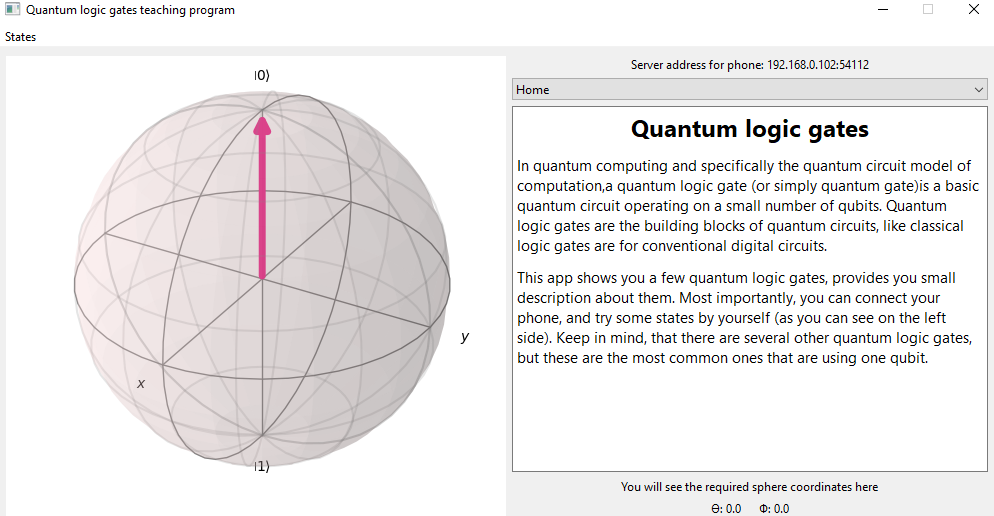
\includegraphics[width=0.6\linewidth]{Program}
	\caption{Az asztali alkalmazás kinézete indításkor}
	\label{fig:program}
\end{figure}

\subsubsection{Menü}
A program tartalmaz egy felső menü sávot, ebben egy States menüponttal. Ezen belül találhatóak az egyes bázisvektor állítási lehetőségek a Bloch gömbhöz. 

\begin{lstlisting}[caption={Menü inicializálása}]
# Menu Bar
self.menu = self.menuBar()
self.menu_states = self.menu.addMenu("States")
self.menu_random = QAction("Random Bloch state", self)
self.zero_state_option = QAction("|0> bloch state", self)
self.one_state_option = QAction("|1> bloch state", self)
\end{lstlisting}

Az összes menüpont kattintással használható. A menü a menuBar, a bázisvektorok menüpontjai pedig a QAction osztályok példányai. A QAction osztály felel a gombok kattintásra történő működéséért, meghívja az adott menüponthoz tartozó eljárást, amennyiben az kiválasztásra került.

\begin{lstlisting}[caption={Menü elemek bekötése}]
# Menu Bar
self.menu_random.triggered.connect(self.__random_state)
self.zero_state_option.triggered.connect(self.__zero_state)
self.one_state_option.triggered.connect(self.__one_state)
self.menu_states.addAction(self.menu_random)
self.menu_states.addAction(self.zero_state_option)
self.menu_states.addAction(self.one_state_option)
self.menu.addMenu(self.menu_states)
\end{lstlisting}

\subsubsection{Bloch gömb}
A Bloch gömb megvalósítása a Qiskit visualization csomagjának segítségével történt. Ez tartalmaz egy plot függvényt, ami egy matplotlib ábrával tér vissza.A programban paraméterei közé tartozik egy három elemű tömb, ami alapján a gömb készül, valamint a koordináta típusa. 

Az elkészült matplotlib ábrát a Pyside FigureCanvasQTAgg osztály egy példányához adom, ezzel egy "vásznat" biztosítva a Bloch gömbnek. Ez a futás során folyamatosan frissül a különböző vektorállapotok miatt.

A vásznat egy QHBoxLayout példányhoz adom, ami horizontálisan jeleníti meg az elemeket.

\begin{lstlisting}[caption={A Bloch gömb kezdő állapota a konstruktorban},label=blochspherestart]
# Bloch sphere part
self.bloch_vector = BlochVector.BlochVector(0.0, 0.0)
self.fig = plot_bloch_vector([1, self.bloch_vector.theta, self.bloch_vector.phi], coord_type='spherical')
self.canvas = FigureCanvasQTAgg(self.fig)
\end{lstlisting}

\subsubsection{Jobb oldali információ panel}
A Bloch gömb mellett a másik legfontosabb rész a felületen.

A panel legfelső részén a szerver ip címe látható, ami a QLabel osztály példánya. A címet az általam létrehozott Server osztály egy példányából nyerem ki.

Ez alatt egy legördülő menü helyezkedik el. A QComboBox példányához hozzáadtam a lehetséges kapu változatokat, illetve egy kezdőoldalt. A menüpont változását folyamatosan ellenőrzi a program, ehhez tartozik egy publikus eljárás, valamint egy változó is. A metódus adott opció alapján alakítja ki a felületet, ez felelős azért, hogy adott kapuhoz a megfelelő információk jelenjenek meg. A változó az ezt követő gombok működése miatt fontos. Az eljárás publikussága a kezdeti állapot beállítás miatt szükséges.

A következő elem a leírás. Ez egy QTextEdit példány, ami tartalmazza az adott kapuk információit. Menüpont váltás miatt folyamatosan cserélődik.

A leíráshoz tartozik egy áramkörrajz a kapuról. Ez az alkalmazás indulásakor nem látszódik, csak amennyiben ellépünk a kezdő oldalról. A rajzot külön generáltattam és lementettem a Qiskit QuantumCircuit csomagjával.

Az áramkör rajzhoz hasonlóan két gomb sem látszódik a kezdő állapotban, amik a QPushButton példányai. Mindkettő függ attól, hogy melyik kapu van kiválasztva. Az első felel az animációs ablak megjelenítéséért. A második gomb lenyomásával a program alkalmazza a kiválasztott kaput a Bloch gömbön és elindít egy forgatási metódust, amennyiben a felhasználó csatlakoztatott telefont. Ha ez nem történt meg, a program egy felugró ablakban figyelmeztet, hogy csatlakoztasson telefont. Az ablak egy QMessageBox példánnyal valósul meg

A panel legalsó részén két QLabel példány látható, amik tartalmazzák a gömb jelenlegi koordinátáit, valamint a forgatás során megjelennek a célkoordináták is.

A felsorolt elemeket egy QVBoxLayout példányhoz adom, ami vertikálisan jeleníti meg őket. Ezt pedig a már említett QHBoxLayout példányhoz adom, hogy a Bloch gömb mellett jelenjen meg.

\begin{lstlisting}[caption={A jobb oldali panel és elemeinek létrehozása a konstruktorban}]
# Right side of the program
self.addr_label = QLabel()
self.gates_combo = QComboBox()
self.info_text = QTextEdit()
self.label = QLabel()
self.pixmap = QPixmap()
self.show_anim = QPushButton()
self.start_measure_button = QPushButton()
self.coordinate_label = QLabel()
self.current_coordinate_label = QLabel()
self.right_side = QVBoxLayout()
self.which_gate = ""
\end{lstlisting}

\begin{lstlisting}[caption={A jobb oldali panel elemeinek értékadása}]
# Right side of the program
self.addr_label.setText("Server address for phone: " + str(server_start.host) + ":" + str(server_start.port))

self.gates_combo.addItems(["Home", "Identity", "Pauli-X", "Pauli-Y", "Pauli-Z", "Hadamard", "Phase", "T"])

self.label.setPixmap(self.pixmap)

self.coordinate_label.setText("You will see the required sphere coordinates here")
self.current_coordinate_label.setText("\u03F4: " + str(self.bloch_vector.theta) + "\t\u03A6: " + str(self.bloch_vector.phi))

self.info_text.setReadOnly(True)
self.label.setVisible(False)
self.show_anim.setVisible(False)
self.start_measure_button.setVisible(False)
\end{lstlisting}

\begin{lstlisting}[caption={Elemek hozzáadása a jobb oldali panelhez, gombok beállítása}]
self.right_side.addWidget(self.addr_label)
self.right_side.addWidget(self.gates_combo)
self.right_side.addWidget(self.info_text)
self.right_side.addWidget(self.label)
self.right_side.addWidget(self.show_anim)
self.right_side.addWidget(self.start_measure_button)
self.right_side.addWidget(self.coordinate_label)
self.right_side.addWidget(self.current_coordinate_label)
self.right_side.setAlignment(self.addr_label, Qt.AlignCenter)
self.right_side.setAlignment(self.label, Qt.AlignCenter)
self.right_side.setAlignment(self.coordinate_label, Qt.AlignCenter)
self.right_side.setAlignment(self.current_coordinate_label,
	Qt.AlignCenter)

self.gates_combo.currentTextChanged.connect(self.gates_combo_options)
self.show_anim.clicked.connect(self.__open_anim_window)
self.start_measure_button.clicked.connect(self.__start_gate_check)
\end{lstlisting}

\subsubsection{Animációs ablak}
A különböző kapukhoz a felhasználó megtekintheti azok animációját is, amely a $\ket{0}$ standard bázisvektorból indul. Ezeket külön kigeneráltattam és kimentettem a Qiskit visualization csomag segítségével. 

Az animáció folyamatosan ismétlődik, amíg a felhasználó be nem zárja a megjelent plusz ablakot, amit a hozzá tartozó gomb lenyomásával érhet el. Kattintáskor egy privát metódus indul, ahol a kiválasztott kapu alapján a program példányosít egy általam létrehozott AnimationWindow osztályt. Az osztály konstruktora a megfelelő gif elérési útvonalát tartalmazza, valamint az ablak szükséges beállításait, illetve egy privát eljárást. A metódus példányosít egy QMovie osztályt, ami a gif megjelenítéséért felel.

\begin{lstlisting}[caption={AnimationWindow osztály}]
class AnimationWindow(QMainWindow):
	def __init__(self, gate, parent=None):
		QMainWindow.__init__(self, parent)
		
		self.setWindowTitle("Gate animation")
		self.setFixedSize(500, 500)
		
		self.gif_label = QLabel(self)
		self.gif_label.setFixedSize(500, 500)
		
		self.gif_path = gate
		
		self.__display_gif()

	def __display_gif(self):
		movie = QMovie(self.gif_path)
		self.gif_label.setMovie(movie)
		movie.start()
\end{lstlisting}

\subsection{Kommunikáció a telefonnal}
Az asztali alkalmazás legérdekesebb része a telefonnal történő vektorforgatás lehetősége. Ehhez szükséges volt a kapcsolat kialakítása egy telefonos applikáció és a program közt.

A hálózat tevékenységeit az általam létrehozott Server osztály egy példánya kezeli. Konstruktora tárolja a host ip címet, valamint a port számot. A host a számítógép címe, a port számot pedig az operációs rendszer választja ki a szabadok közül.

\begin{lstlisting}[caption={A Server osztály konstruktora}]
def __init__(self, HOST, PORT):
	self.s = socket.socket(socket.AF_INET, socket.SOCK_STREAM)
	self.host = HOST
	self.port = PORT
	self.s.bind((self.host, self.port))
	self.port = self.s.getsockname()[1]
	self.conn = ""
	self.addr = ""
\end{lstlisting}

\subsubsection{Szerver indítása és kapcsolat várása}
A Window osztály példányosítása előtt a program elindít egy metódust, amiben egy PhoneConnector osztály példánya foglal helyet. 

A példány threading segítségével a háttérben elindítja egyetlen metódusát. Ennek köszönhetően a szerver elindul és várja a telefon csatlakozását. Egy felugró ablak jelzi ennek sikerességét, amit pedig egy Signal példány hív meg. Egyszerre csak egy telefont tud csatlakoztatni a felhasználó, ezt a Server osztály példányának metódusa ellenőrzi.

\begin{lstlisting}[caption={A Window osztály példányosítása előtt elindított metódus}]
def connect_phone():
	phone_connector = PhoneConnector()
	phone_connector.connected.connect(show_phone_connected_message)
	phone_thread = threading.Thread(target=phone_connector.run)
	phone_thread.start()
\end{lstlisting}

\begin{lstlisting}[caption={PhoneConnector osztály}]
class PhoneConnector(QObject):
	connected = Signal()

	def run(self):
		if server_start.hosting():
			self.connected.emit()
\end{lstlisting}

\begin{lstlisting}[caption={A csatlakozást váró függvény a Server osztályban}]
def hosting(self):
	self.s.listen(0)
	self.conn, self.addr = self.s.accept()
	return True
\end{lstlisting}

\subsubsection{Szenzor adatok fogadása és tárolása}
A telefon szenzor adatait az asztali alkalmazás a forgatás pillanatában kezdi el fogadni és egy tömbben tárolni. 

Mivel a telefon már a csatlakozás pillanatában is próbálja küldeni az adatokat, így az első csomag amit fogad a program, eldobásra kerül, csakúgy, mint azok az adatok, amik nem két elemű float tömböt adnak. A felhasználó ezeket az adatvesztéseket nem érzékeli, esetleg a vektor forgatásának lassabb folyamata látszódhat.

Amennyiben a kapcsolat megszűnik, a program üres csomagot fog kapni. Ebben az esetben a szerver bontja a kapcsolatot a klienssel. Amint ez megtörténik, a szerver újra elkezdi várni a kapcsolatot és kezdődik az elejéről a folyamat.

\begin{lstlisting}[caption={Szenzor adatok fogadása és tárolása valamint kapcsolat bontása}]
def get_data(self):
	data = self.conn.recv(1024).decode()
	if not data:
		self.conn.close()
		return None
	else:
		angles = data.split(',')
		return angles
\end{lstlisting}

\subsection{Matematikai számítások}
Ugyan a felhasználó nem érzékeli, de a program jelentős része háttérszámításokon alapul. Ehhez kialakítottam egy BlochVector osztályt, ahol az adott gömbkoordináták alapján tud az alkalmazás számításokat végezni.

\subsubsection{Gömbkoordináták}
A bejövő szenzor adatok és a számítások egyszerűsítése miatt gömb koordináta-rendszert használtam. Amennyiben ezt nem adom meg a Bloch gömb rajzolásakor, a Qiskit automatikusan a másik opciót, azaz a  Descartes-féle koordináta rendszert használja. Ennek megfelelően a paraméterében a három elemű tömb tartalma rendre (ami \az{\ref{blochspherestart}}.~kódban is látható):

\begin{enumerate}
	\item Az origótól mért távolság, tehát a gömb sugara. Ez jelen esetben mindig egy lesz. Jele: $r$
	\item Azimut szög, azaz a pont és a $\phi=0$ tengely által meghatározott sík, valamint $\theta=0$ sík közötti hajlásszög az $x-y$ koordinátasíkban. Jele: $\theta$
	\item A pontot és az origót összekötő egyenes hajlásszöge a $\phi=0$ irányhoz, azaz az $z$ tengellyel bezárt szög. Jele: $\phi$
\end{enumerate}

Mivel a gömb sugara nem változik, így a továbbiakban csak a $\theta$ és a $\phi$ értékei változnak.

A Qiskit csomagja mellett létrehoztam egy BlochVector osztályt, mely konstruktorában tárolja a szükséges értékeket a későbbi számításokhoz, megjelenítésekhez.

\subsubsection{Standard- és véletlenszerű bázisvektorok generálása}
Az alkalmazás menüsávjában a felhasználó kiválaszthatja, hogy milyen bázisvektor állást szeretne magának a gömb forgatása előtt használni. A kiválasztott opció elindítja az ahhoz tartozó eljárást, ami beállítja a Bloch gömb állapotát.

A véletlenszerű generálás esetén a metódus $\theta$ értékét 0 és $\pi$ között, $\phi$~-t pedig 0 és $2\pi$ közt határozza meg, a gömbkoordináta szabályainak megfelelően.

Az említett szabályok alapján a $\ket{0}$ állapot $\theta=0$ $\phi=0$, $\ket{1}$ pedig $\theta=\pi$ $\phi=0$ állapotot fog kapni.

A megadott koordinátákon kívül nincs különbség a három eljárásban, viszont a gombok és egyéb hívások miatt átláthatóbb opció volt ezeket nem egy metódusban tartani.

\begin{lstlisting}[caption={Véletlenszerű bázisvektor generálása és Bloch gömb rajzolása}]
def __random_state(self):
	# Set Bloch sphere to a random state
	self.bloch_vector.theta = random.uniform(0.0, np.pi)
	self.bloch_vector.phi = random.uniform(0.0, 2 * np.pi)
	plt.close()
	self.fig.canvas.flush_events()
	self.fig = plot_bloch_vector([1, self.bloch_vector.theta, self.bloch_vector.phi],
	coord_type='spherical')
	self.canvas.figure = self.fig
	self.fig.set_canvas(self.canvas)
	self.canvas.draw()
	self.current_coordinate_label.setText("\u03F4: " + str(self.bloch_vector.theta)
	+ "\t\u03A6: " + str(self.bloch_vector.phi))
\end{lstlisting}


\subsubsection{Bázisvektor mátrix kialakítása gömbkoordináták alapján}
A kigenerált bázisvektorral a program forgatás kezdésekor kezd el foglalkozni. Ekkor a BlochVector osztálynak egy olyan privát függvénye is lefut, ahol a már ismert $\theta$ és $\phi$ értékeiből kiszámítjuk $\alpha$ és $\beta$ értékeit, amit egy mátrixban tárolunk. Mivel a bázisvektor egy qubit állapotát jelenti, így \az{\ref{qubitallapot}}., valamint \az{\ref{qubitallapothelyettesit}}.~képletekből indulhatunk ki.

\begin{equation}\label{qubitallapothelyettesit}
	\ket{\Psi}=\cos\frac{\theta}{2}\ket{0}+e^{i\phi}\sin\frac{\theta}{2}\ket{1},
\end{equation}

ahol $i$ komplex szám, $\theta$ és $\phi$ pedig a már említett gömbkoordináták.

\begin{lstlisting}[caption={Bázisvektor mátrix kialakítása a képletek alapján}]
def __start_state_vector(self):
	alpha = np.cos(self.theta / 2)
	beta = np.exp(1j * self.phi) * np.sin(self.theta / 2)
	state_vector = np.array([[alpha], [beta]])
	return state_vector
\end{lstlisting}

\subsubsection{Kapuk alkalmazása a bázisvektor mátrixán}
A kapott bázisvektor mátrixon szorzást hajt végre a program, az alapján, hogy melyik kapu lesz kiválasztva. Ahogy azt a \ref{kvantumkapuk}.~fejezetben láttuk, mindegyik kvantumkapu egyedi mátrix-val rendelkezik. A szorzás által kapott mátrix lesz az új bázisvektor mátrixa.

\begin{lstlisting}[caption={Pauli-X kapu alkalmazása a bázisvektorra}]
def pauli_x(self):
	pauli_x_matrix = np.array([[0, 1], [1, 0]])
	state_vector_after_gate = np.dot(self.__start_state_vector().T, pauli_x_matrix)
	coordinates = get_spherical_coordinates_from_state_vector(state_vector_after_gate)
	self.theta = coordinates[0]
	self.phi = coordinates[1]
\end{lstlisting}

\subsubsection{Új bázisvektor számítása}
\Az{\ref{qubitallapot}}.~képlet felírható polár alakban:

\begin{equation}
	\ket{\Psi}=(r_\alpha)e^i(\phi a)\ket{0}+(r_\beta)e^i(\phi b)\ket{1}
\end{equation}

Ebben a formában négy változó van, két valós szám és két képzetes. Ezekből kiindulva az alábbi kód alapján történik théta és fí visszafejtése az új bázisvektorból. Ezeket az adatokat küldi tovább a program a forgatás ellenőrzéséhez.

\begin{lstlisting}[caption={Fí és théta kinyerése az új bázisvektorból}]
def get_spherical_coordinates_from_state_vector(state_vector_after_gate):
	alpha_real = state_vector_after_gate[0][0].real
	alpha_imag = state_vector_after_gate[0][0].imag
	beta_real = state_vector_after_gate[0][1].real
	beta_imag = state_vector_after_gate[0][1].imag
	
	if alpha_real != 0.0:
		if alpha_real < 0 < alpha_imag:
			alpha_theta = np.arctan(alpha_imag / alpha_real) + np.pi
	
		elif alpha_real < 0 and alpha_imag < 0:
			alpha_theta = np.arctan(alpha_imag / alpha_real) + np.pi
		else:
			alpha_theta = np.arctan(alpha_imag / alpha_real)
	else:
		alpha_theta = 0.0
	
	r_alpha = np.sqrt((alpha_real ** 2) + (alpha_imag ** 2))
	
	if beta_real != 0.0:
		if beta_real < 0 < beta_imag:
			beta_theta = np.arctan(beta_imag / beta_real) + np.pi
	
		elif beta_real < 0 and beta_imag < 0:
			beta_theta = np.arctan(beta_imag / beta_real) + np.pi
		else:
			beta_theta = np.arctan(beta_imag / beta_real)
	else:
		beta_theta = 0.0
	
	theta = 2 * np.arccos(r_alpha)
	phi = beta_theta - alpha_theta
	if phi < 0:
	phi += 2 * np.pi
	coordinates = [theta, phi]
	return coordinates
\end{lstlisting}

\subsection{Vektor forgatása és ellenőrzése}
Az előző alfejezetekben tárgyalt elemei az asztali alkalmazásnak, mind hozzásegítenek ehhez a funkcióhoz. A csatlakoztatott telefonnal a felhasználó alkalmazhat egy kaput a kvantumbiten. Amint a háttérszámítások alapján előáll az új bázisvektor, elkezdődik a forgatás, amiért egy privát metódus felel, ahol egy ciklus fut az új állapot eléréséig, vagy hibáig.

\subsubsection{Tárolt szenzor adatok feldolgozása}
A ciklus folyamatosan kéri az új szenzor adatokat. Ha üres tömböt kap, egy felugró ablak üzenete után a gömböt $\ket{0}$ állapotba állítja, újra kapcsolatot vár és kilép a ciklusból, ezzel együtt az eljárásból is.

Ellenkező esetben a kapott adatokat ellenőrzi. Ha a tömb nem két elemű, valamint nem lehet float típusúvá konvertálni, akkor az adatot "eldobja", folytatja a következő érkezett adattal.

Ezután a beérkezett szenzor adatok közül $\phi$ értékét módosítjuk, hogy 0 és $2\pi$ érték között legyen.

\begin{lstlisting}[caption={Tárolt szenzor adatok feldolgozása}]
while True:
	angles = server_start.get_data()
	if angles is None:
		show_message("Phone disconnected! Please reconnect to continue!")
		self.__zero_state()
		connect_phone()
		break
	else:
		try:
			angles = np.array(angles, dtype=float)
			if angles[1] < 0:
				angles[1] = angles[1] + 2 * np.pi
\end{lstlisting}

\subsubsection{Bloch gömb újrarajzolása}
Minden új adatnál, a gömb újrarajzolásra kerül. Az előtte megjelenített rajz, valamint a vászon törlésre kerül, memória- és helyfelszabadítás miatt. Helyére egy új gömb jut, ahol $\theta$ és $\phi$ értéke az új szenzoradatokra cserélődik.

\begin{lstlisting}[caption={Bloch gömb újrarajzolása}]
plt.close()
self.fig.canvas.flush_events()
self.fig = plot_bloch_vector([1, angles[0], angles[1]], coord_type='spherical')
self.canvas.figure = self.fig
self.fig.set_canvas(self.canvas)
self.canvas.draw()
\end{lstlisting}


\subsubsection{Gömbkoordináta ellenőrzése}
A Bloch gömb kirajzoltatása után a ciklus végén ellenőrzi a program, hogy a jelenlegi vektor állása megfelel-e a kvantumkapu alkalmazásával kapott bázisvektornak. Az egyszerűbb működés érdekében ez 0.1 relatív- és 0.15 abszolút toleranciával működik. Ha a felhasználó ezeken belül van, a program egy felugró ablakban jelzi hogy megtalálta a keresett bázisvektort és a ciklus leáll. Ezután újra elvégezheti a műveletet, de akár más kaput is választhat, mindaddig, amíg a telefon csatlakoztatva marad.

\section{Applikáció bemutatása}
Mivel a hangsúly elsősorban az asztali alkalmazáson van, így az android applikáció egy egyszerű megvalósítást képvisel, viszont hasonlóan az elképzelések alapján készült, valamint bővíthető.

\subsection{Grafikus felhasználói felület}
A grafikai elemek megjelenítéséért elsődlegesen egy xml fájl felel, amit az Android Studio automatikusan létrehoz az egyes activity-khez. Itt adhatjuk meg az egyes elemeket, akár kódként, de lehetséges a Design panelen behúzni őket az applikáció felületére.

\begin{figure}[H]
	\centering
	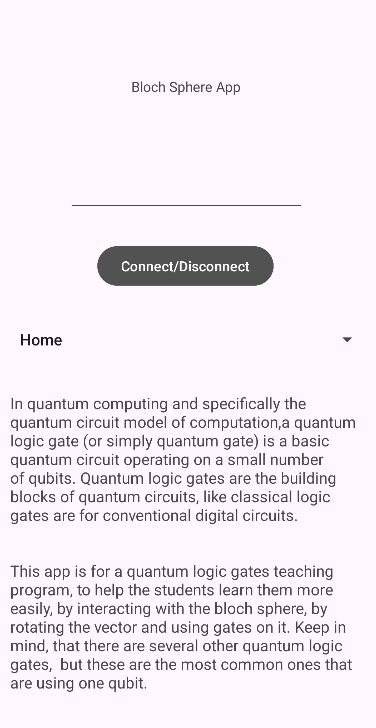
\includegraphics[width=0.25\linewidth]{app}
	\caption{Az applikáció kinézete indításkor}
	\label{fig:app}
\end{figure}

Az applikáció tartalmaz egy EditText elemet, ahova a felhasználó a csatlakozási címet írhatja be. Ez csak akkor elérhető, ha a telefon még nem csatlakozott az asztali alkalmazáshoz.

Ehhez tartozik egy gomb, ami a csatlakozást/lecsatlakozást kezeli. Ez befolyásolja többek között az EditText elem elérhetőségét is, de elsősorban nem ez a célja.

\begin{lstlisting}[caption={Button létrehozása xml-ben}]
<Button
	android:id="@+id/button"
	android:layout_width="wrap_content"
	android:layout_height="wrap_content"
	android:backgroundTint="#535252"
	android:text="Connect/Disconnect"
	app:layout_constraintBottom_toBottomOf="parent"
	app:layout_constraintEnd_toEndOf="parent"
	app:layout_constraintHorizontal_bias="0.497"
	app:layout_constraintStart_toStartOf="parent"
	app:layout_constraintTop_toTopOf="parent"
	app:layout_constraintVertical_bias="0.358" />
\end{lstlisting}

Mivel fontos volt, hogy az asztali alkalmazáson elért rövid információk elérhetőek legyenek a telefonon is, ezért ezt egy Spinner, TextView és egy ImageView elemmel valósítottam meg. Előbbihez az activity-hez tartozó java fájlban hozzáadtam egy tömböt, ami tartalmazza az egyes menüpontokat. Tartozik még ehhez továbbá egy Listener eljárás, ahol az applikáció folyamatosan figyeli, hogy a felhasználó mikor vált menüpontot és ennek megfelelően változtatja a felületet. Az ImageView a főmenüben nem látszik, kapu kiválasztáskor jelenik meg. A leírást tartalmazó elemhez hasonlóan a felület legfelső részén elhelyezkedő cím is TextView elem.


Az xml-ben felsorolt elemek a cím TextView-n kívül a java fájlban példányosítva vannak, az azokkal történő műveletek miatt. Ugyanitt fontos megjegyezni, hogy az applikáció nem lép alvó módba. Ezt egy flag-vel értem el, ami az activity ablakához adódik, egy konstans értékkel.

\subsection{Kommunikáció az asztali alkalmazással}

\subsection{Szenzor adatok gyűjtése}
Miután a telefon sikeresen csatlakozott az asztali alkalmazáshoz, az applikáció példányosít egy SensorManager osztályt, ez felel a szenzorok létrehozásáért, valamint fel- és leregisztrálásáért.

Miután a példányosítás megtörtént, a program létrehoz egy szenzort és regisztrálja azt. Az Android Studio számos szenzortípussal szolgál, ezek mind különböző feladatot látnak el. A forgatás szempontjából számunkra az Orientation szenzor típus a megfelelő. Regisztráláskor fontos megadni a szenzoradat késleltetés idejét. Ez lehet beépített konstans érték, de lehet általunk megadott egyedi érték is. 

\begin{lstlisting}[caption={Szenzor létrehozása és regisztrálása}]
sensorManager = (SensorManager) getSystemService(Context.SENSOR_SERVICE);
sensor = sensorManager.getDefaultSensor(Sensor.TYPE_ORIENTATION);
sensorManager.registerListener(MainActivity.this,sensor,SensorManager.SENSOR_DELAY_NORMAL);
\end{lstlisting}

A MainActivity osztály implementál egy SensorEventListener osztályt, ami tartalmaz egy publikus eljárást, ahol a szenzor változást figyelhetjük. Ebben a metódusban tároljuk a szükséges $\theta$ és $\phi$ értékét, majd a már említett PrintWriter példánnyal küldjük az adatokat az asztali alkalmazás számára.

\begin{lstlisting}[caption={Szenzor adatok gyűjtése és küldése az asztali alkalmazás számára}]
@Override
public void onSensorChanged(SensorEvent event) {
	angles =  event.values[0] + "," +
	event.values[2] * 2;
	outToServer.print(angles);
	outToServer.flush();
}
\end{lstlisting}

Kapcsolat bontása esetén a SensorManager példány leregisztrálja a szenzort, és a folyamat kezdődik elölről.

\section{Tesztelések}

\section{Továbbfejlesztési lehetőségek}
Egyik program vagy applikáció sem lehet teljesen kész és hibátlan. Mindig keletkeznek új elképzelések, amik részben, de az is lehet, hogy jelentősen megváltoztatják koncepciót.
\subsection{Részletes matematikai egyenletek mutatása}
A program jelenleg mindent a háttérben számít, a felhasználó semmit nem érzékel ebből. Egy külön textbox-ban meg lehetne jeleníteni az adott qubit egyenletét, valamint annak változását különböző állapotokra, kapukra.

\subsection{Saját áramkör kialakítása}
A legtöbb kvantumkapuval foglalkozó szimulátort sajátosan kialakítható áramkörök szimulálására tervezték. Ezek általában behúzható kapukat tartalmaznak, mindegyik mellé rövid leírás társul. A felhasználó így tetszőleges kvantumáramköröket alakíthat ki, ezzel még jobban érzékelve a kvantumbitek reakcióját bizonyos kapuk alkalmazására.

\begin{figure}[H]
	\centering
	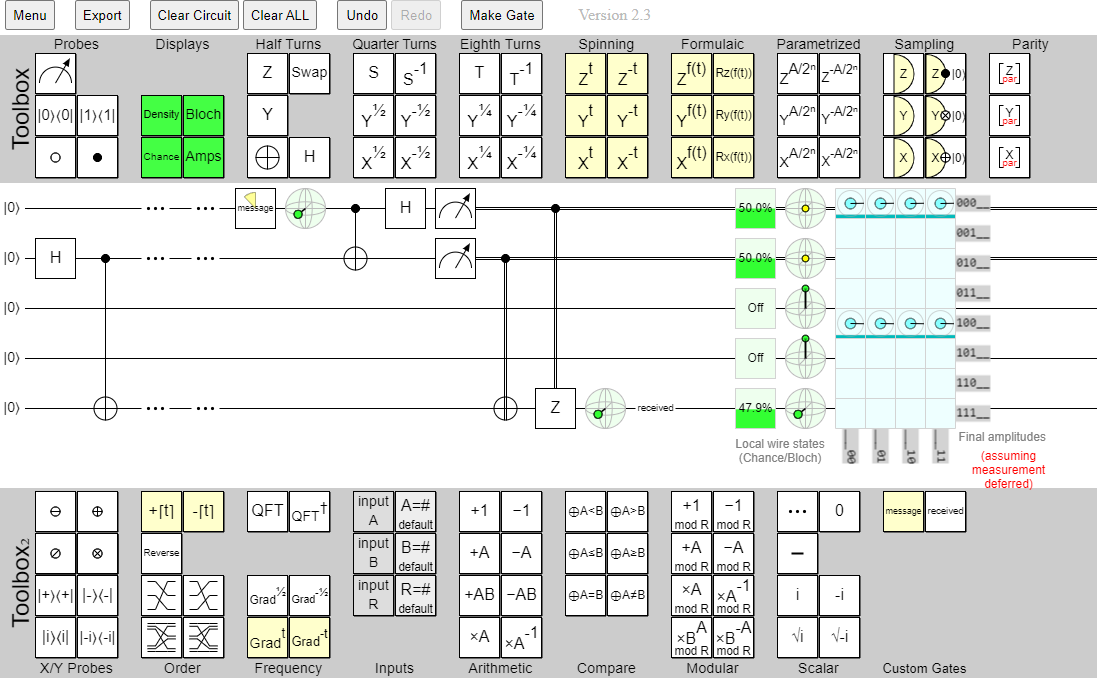
\includegraphics[width=0.5\linewidth]{Simulation}
	\caption{Quirk, az egyik legismertebb webes szimulátor}
	\label{fig:simulation}
\end{figure}

\Az{\ref{fig:simulation}}.~ábrán látható szimulátorhoz hasonlóan a programba is beemelhető lehet egy hasonló megvalósítás, mivel a Qiskit a saját áramkör kialakításban és szimulálásban a legerősebb. Ez ötvözhető lehet a forgatás ellenőrzéssel, amennyiben az áramkörök kialakítását egy kvantumbitre és kapukra korlátozzuk.

\subsection{Több kvantumbites kapuk}
Jelen szakdolgozat ugyan csak egy qubites kapukkal foglalkozik, felmerült hogy későbbiekben ez kibővüljön több kvantumbitre is. Ezek a kapuk ugyanúgy megkapnák azokat az animációkat és pontos ismertetőket.

Ennek a lehetőségnek kihívása az, hogy a jelenleg elérhető Bloch gömb vizualizációkkal körülményes egy olyan forgatás ellenőrzést létrehozni, mint ahogy azt az egy kvantumbites változatoknál láttuk.

Viszont ettől függetlenül a Qiskit lehetőséget nyújt a több kvantumbites kapuk áramkörben történő megjelenítésére és szimulálására. Ezt egy részletes leírással ötvözve szintén egyszerűbb megértést nyújthat a kvantumkapukhoz.

\subsection{Diagramok}
A Qiskit erősségei közé tartoznak még a szimuláció során kinyerhető adatok, amiket diagramok formájában is megjeleníthetünk. Amennyiben ezt ötvözzük a tetszőleges áramkörök lehetőségével, akkor képes lehet a felhasználó látni, hogy bizonyos helyzetekben hogyan reagálnak a kvantumbitek.

Forgatás szempontjából ez az opció kifejezetten memóriaigényes, mivel csakúgy mint a programban lévő Bloch gömb, a diagramok is folyamatos újrarajzolást igényelnének minden új beérkező szenzor adat után.

\subsection{Könyvtárak frissen tartása}
Ahogy a kvantuminformatika, úgy az ezzel foglalkozó Python könyvtárak is rohamosan fejlődnek. A Qiskit jelenleg az 1.0 verziójánál tart és folyamatosan újabb lehetőségekkel, megoldásokkal bővítik könyvtárukat. Ebből adódóan bármikor érkezhet olyan megoldás, ami hozzátenne a programhoz, esetleg hatékonyabbá tenné azt.

\subsection{IOS applikáció}
Az applikáció jelenleg csak androidos telefonokra elérhető, viszont az IOS lehetőséggel több emberhez el tudna jutni a program. Nehézsége, hogy IOS applikációkat MacOSX környezetben lehet csak fejleszteni. Számos megoldás létezik erre a problémára, például a VirtualBox vagy a VMWare, amik virtuális számítógépek kialakítását teszik lehetővé.

\chapter*{Összegzés}
\addcontentsline{toc}{chapter}{Összegzés}


\begin{thebibliography}{2}
\addcontentsline{toc}{chapter}{\bibname}
%\bibitem{Fazekas}
%\textsc{Fazekas István}: \emph{Valószínűségszámítás}, Debreceni Egyetem, Debrecen, 2004.
%\bibitem{Tomacs}
%\textsc{Tómács Tibor}: \emph{A valószínűségszámítás alapjai}, Líceum Kiadó, Eger, 2005.
\end{thebibliography}

% Aláírt, szkennelt nyilatkozat beillesztése a szakdolgozat végére
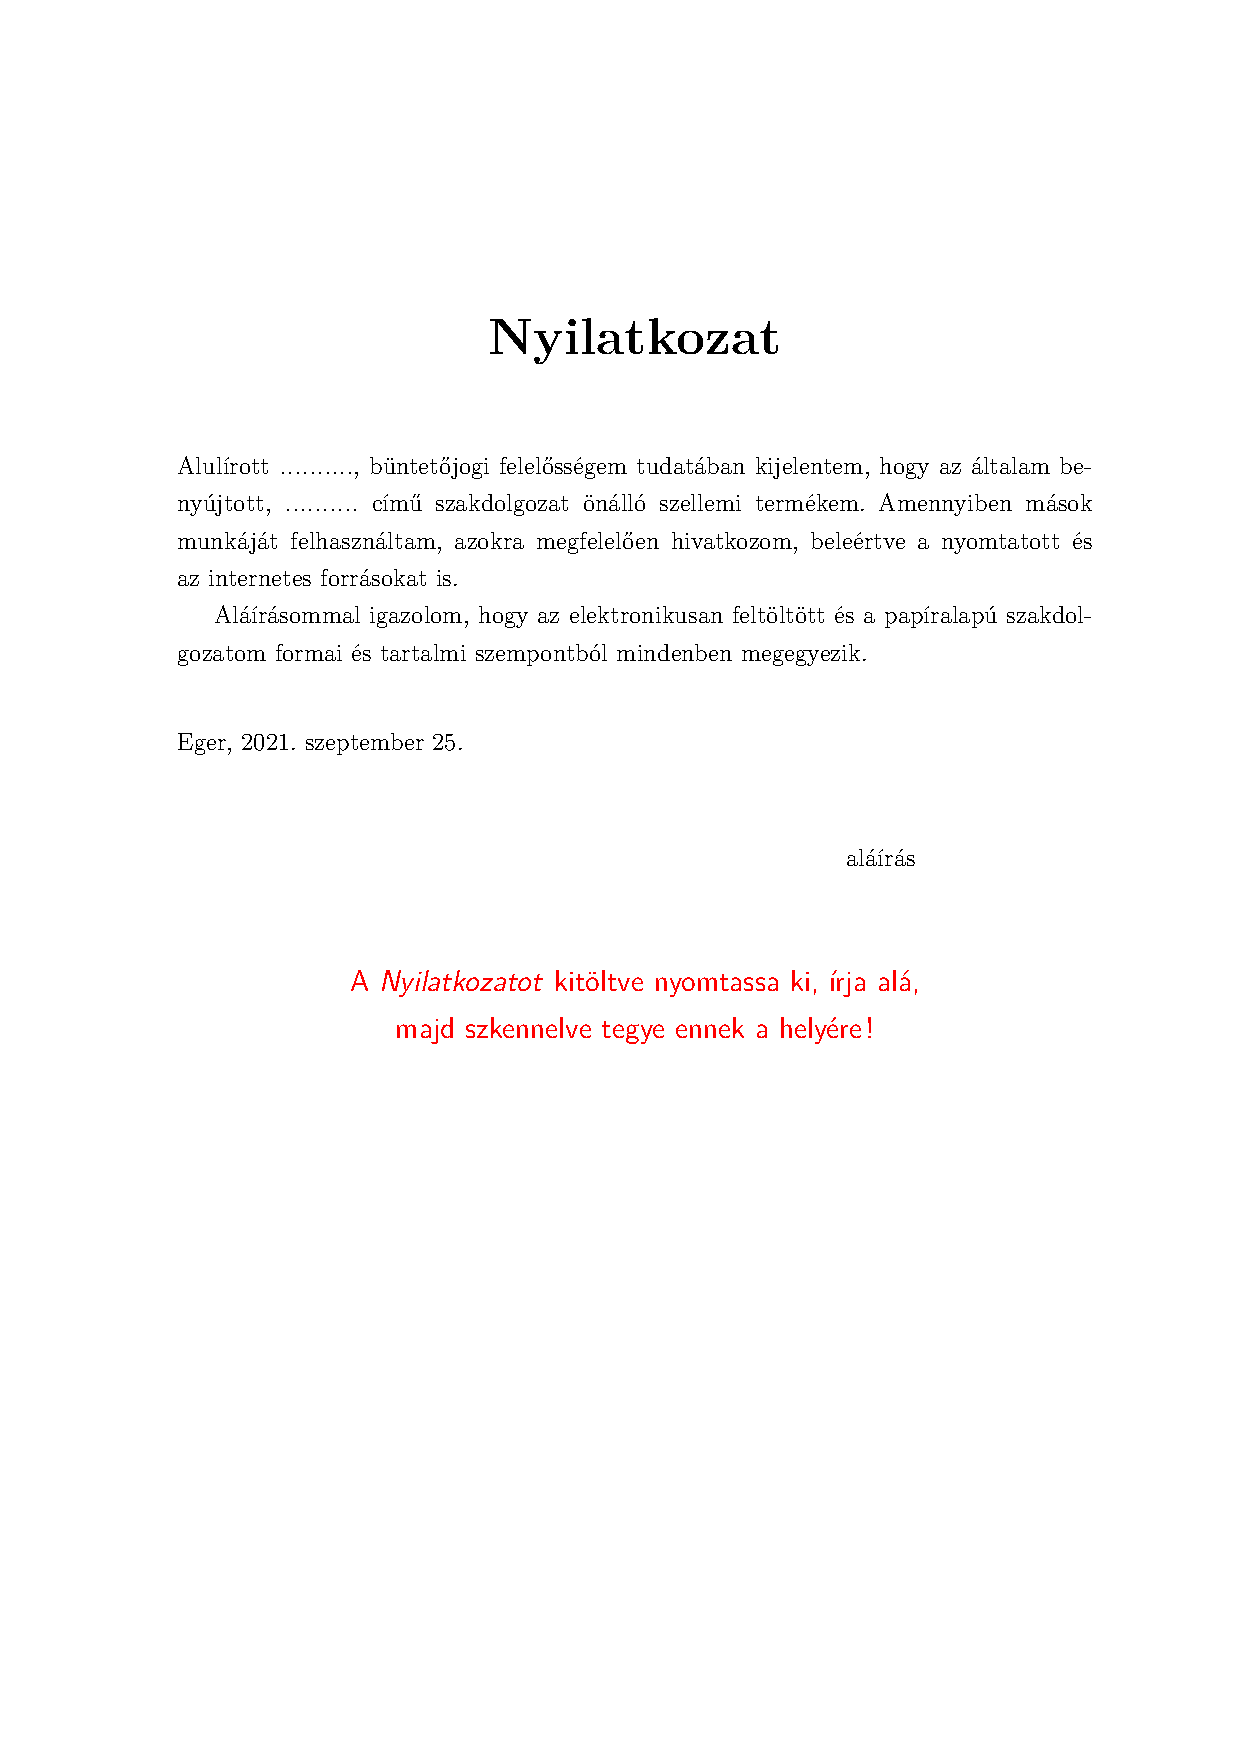
\includepdf{nyilatkozat.pdf}
\end{document}